\documentclass{article}
\usepackage{graphicx} % Required for inserting images
\usepackage{amssymb}
\usepackage[margin=3cm]{geometry}
\usepackage{amsmath}
\usepackage{enumitem}
\usepackage{accents}
\usepackage{wasysym}
\usepackage{cancel}
\usepackage{hyperref}

\renewcommand{\figurename}{Figura}

\title{$\partial d$b$6$}
\author{Samuel Fernández Riquelme}
\date{October 2023}

\begin{document}

\maketitle

\section{Introduction}

\textbf{Problema:} Una sucesión $(a_n)_n$ es contractiva si $|a_{n + 1} - a_n| \leq c|a_n - a_{n - 1}|$, con $0 < c < 1$. Demostrar que si una sucesión es contractiva, entonces es convergente. \\

\textbf{Demostración:} Empezamos observando que si la sucesión es contractiva, entonces $|a_{n + 1} - a_n| \leq c^{n}|a_1 - a_0|$ (asumiendo que empieza en $n = 0$). Esta propiedad se puede deducir de la definición trivialmente, por lo que se deja como ejercicio.

A partir de este punto, nuestro objetivo va a ser llegar a la conclusión de que toda sucesión contractiva es de Cauchy, y, por un resultado visto en clase, también convergente. Por definición, una sucesión es de Cauchy cuando 

\[\forall\varepsilon > 0, \exists n_0 \in \mathbb{N}: n,m \geq n_0 \Longrightarrow |a_m - a_n| < \varepsilon\]

Otra propieda bastante lógica que se podría probar por inducción es, $a_m - a_n$ = $\sum_{i = n}^{m - 1} a_{i + 1} - a_i$, para $m \geq n$. Por tanto, $|a_m - a_n| = |\sum_{i = n}^{m - 1} a_{i + 1} - a_i|$, además, aplicando la desigualdad triangular, $|\sum_{i = n}^{m - 1} a_{i + 1} - a_i| \leq \sum_{i = n}^{m - 1} |a_{i + 1} - a_i|$, asimismo, usando la primera observación, $\sum_{i = n}^{m - 1} |a_{i + 1} - a_i| \leq \sum_{i = n}^{m - 1} c^{i}|a_1 - a_0| = |a_1 - a_0|·\sum_{i = n}^{m - 1} c^{i} = |a_1 - a_0|·(\sum_{i = 0}^{m - 1} c^{i} - \sum_{i = 0}^{n} c^{i})$.

Otro resultado útil es que $\sum_{i = 0}^{n} c^{i} = \frac{1 - c^{n + 1}}{1 - c}$ y para $0 < c < 1$ también cumple $\frac{1 - c^{n + 1}}{1 - c} < \frac{1}{1 - c}$; por tanto, $|a_1 - a_0|·(\sum_{i = 0}^{m - 1} c^{i} - \sum_{i = 0}^{n} c^{i}) < |a_1 - a_0|·(\frac{1}{1 - c} - \frac{1 - c^{n + 1}}{1 - c})$. Además, resulta que $(\frac{1 - c^{n + 1}}{1 - c})_n \longrightarrow \frac{1}{1 - c}$, por lo que la diferencia $\frac{1}{1 - c} - \frac{1 - c^{n + 1}}{1 - c}$ siempre se va a poder hacer todo lo pequeña que uno quiera y, en concreto, más pequeña que un dado $|a_1 - a_0|·\varepsilon$, con $\varepsilon > 0$. 

Esto es equivalente a la definición de sucesión de Cauchy, permitiéndonos asegurar que, efectivamente, una sucesión contractiva es de Cauchy y, consecuentemente, convergente.

\newpage

\section{Ejercicio 7}

Sean $b_i, 1 \leq i \leq n, n > 1$, numeros reales positivos cuyo producto es 1.

\begin{itemize}
    \item[$a)$] Demuestre que si no todos los $b_i$ son iguales y se suponen ordenados de forma creciente,
    $b_1 \leq b_2 \leq ... \leq b_n$, entonces $b_1 < 1 < b_n$.

    \vspace{7px}

    \textsc{Demostración}: Supongamos, de manera absurda, que $b_1 \geq 1$ o que $b_n \leq 1$. Únicamente se detalla el razonamiento para el primer escenario, quedando a elección del lector si decide darle el cierre que se merece a esta prueba.

    Bien, supuesto $b_1 \geq 1$ y sabiendo que no todos son iguales, adquirimos $b_n > 1$, por lo que llegamos a

    \[b_1b_2...b_n = (b_1b_2...b_{n-1})b_n \geq 1 \cdot b_n > 1,\]

    de donde la contradicción aflora de forma radiante. \hfill{\textsc{Q.e.d.}}

    \item[$b)$] Utilizando inducción en $n$, pruebe que
    
    \begin{equation}
        b_1b_2...b_n = 1 \leq \frac{b_1 + b_2 + ... + b_n}{n},
        \label{eq:agm}
    \end{equation}

    y que solo se tiene la igualdad cuando todos los $b_i$ son iguales.

    \vspace{7px}

    \textsc{Demostración}: Creo que nada ha de decirse respecto a la obviedad de que, en \eqref{eq:agm}, la igualdad al menos ocurre cuando los $b_i$ comparten el mismo valor, es decir, 1.
    Por tanto, de aquí en adelante asumimos que no son enteramente iguales y nos las apañaremos para fundamentar la desigualdad estricta.

    Procedamos con la inducción:

    \begin{itemize}
        \item \textbf{Caso base}: $n = 2$. Simplemente nos limitamos a estudiar la desigualdad
        
        \[1 = b_1b_2 = \sqrt{b_1b_2} < \frac{b_1 + b_2}{2},\]

        de la siguiente manera:

        \[\sqrt{b_1b_2} < \frac{b_1 + b_2}{2} \iff b_1b_2 < \frac{(b_1 + b_2)^2}{4}\]
        \[\hspace{100px} \iff 4b_1b_2 < b_1^2 + 2b_1b_2 + b_2^2\]
        \[\hspace{83px}\iff b_1^2 - 2b_1b_2 + b_2^2 > 0\]
        \[\hspace{65px}\iff (b_1 - b_2)^2 > 0,\]

        lo cual es siempre cierto bajo las hipótesis impuestas (i.e. $b_1 \neq b_2$). Nótese que, en verdad, lo que hemos probado es que para cualesquiera $x, y \in \mathbb{R}^+$ distintos se tiene que $\sqrt{xy} < (x + y) / 2$.

        \item \textbf{Paso inductivo}. Supongamos que, para $n$ reales postivos $a_1, a_2, ..., a_n$ (no todos iguales) arbitrarios tales que $a_1a_2...a_n = 1$, se cumple que
        
        \begin{equation}
            n < a_1 + a_2 + ... + a_n.
            \label{eq:agmstrc}
        \end{equation}

        A continuación, considerando $n + 1$ reales positivos ordenados $b_1b_2...b_{n+1}$ (no todos iguales) cuyo producto es $1$, veamos que se satisface $n + 1 < b_1 + b_2 + ... + b_{n + 1}$. Para ello, construimos la secuencia de números auxiliares $a_1, a_2, ..., a_n$ tales que

        \[
        a_k := 
        \begin{cases}
            b_1b_{n + 1} & \text{si $k = 1$} \\
            b_k & \text{si $1 < k \leq n$}
        \end{cases}
        .\]

        De esta manera, es evidente que su producto sigue valiendo $1$. No obstante, tenemos que diferenciar dos casos, pues puede suceder que después de hacer este
        agrupamiento todos los $a_i$ valgan $1$. En dicho escenario, se tiene trivialmente que $n = a_1 + a_2 + ... + a_n$, mientras que si no se da esta condición aplicamos 
        la hipótesis de inducción para alcanzar \eqref{eq:agmstrc}. En definitiva, no importa el escenario, sabemos que

        \[n \leq a_1 + a_2 + ... + a_n = b_1b_{n+1} + b_2 + ... + b_n.\]

        Pero está claro que aún no hemos terminado. Si tan sólo se pudiese afirmar que $1 < b_1 + b_{n + 1} - b_1b_{n + 1}$... Un momento, pero si sí que se puede, ¡allá que vamos pandilla!

        Teniendo presente en mente que $b_1 < 1 < b_{n + 1}$ por el apartado anterior, notamos que 

        \[1 < b_{n + 1} \Longrightarrow 1 - b_1 < b_{n + 1}(1 - b_1),\]

        pues $1 - b_1 > 0$, y de aquí llegamos a que

        \[1 < b_1 + b_{n + 1} - b_1b_{n + 1}.\]

        Los restantes y vagos argumentos se confían al rector. \hfill{\textsc{Q.e.d.}}
    \end{itemize}

    \item[$c)$] Deduzca que si $a_i > 0, 1 \leq i \leq n$, son números reales, entonces
    
    \[\sqrt[n]{a_1a_2...a_n} \leq \frac{a_1 + a_2 + ... + a_n}{n}.\]

    \vspace{7px}

    \textsc{Solución}: Denotemos mediante $x \in \mathbb{R}$ a la media geométrica de los $a_i$, o más llanamente

    \[x := \sqrt[n]{a_1a_2...a_n}.\]

    Considerando los términos $b_i = a_i / x$, a poco que lo pienses, llegamos a que

    \[\sqrt[n]{b_1b_2...b_n} = 1\]

    o, lo que es lo mismo, que el producto de los $b_i$ es $1$, por lo que estamos en condiciones de invocar el resultado del apartado $b)$. En consecuencia, obtenemos que

    \[\frac{\sqrt[n]{a_1a_2...a_n}}{x} = \sqrt[n]{b_1b_2...b_n} = 1 \leq \frac{b_1 + b_2 + ... + b_n}{n},\]

    y, pasando la $x$ multiplicando, concluimos finalmente que

    \[\sqrt[n]{a_1a_2...a_n} \leq \frac{x(b_1 + b_2 + ... + b_n)}{n} = \frac{a_1 + a_2 + ... + a_n}{n}.\]

    $\hfill\square$
\end{itemize}

\newpage

\section{Ejercicio 22*}

Sean $A$ y $B$ dos subconjuntos no vacíos de $\mathbb{R}$. Se definen

\[A + B = \{x = a + b : a \in A, b \in B\}, -A = \{x = -a : a \in A\}\]

$a)$ Supongamos que $A, B$ están acotados superiormente. Sabemos que existen $x, x' \in \mathbb{R}$ tal que $a \leq x, \forall a \in A$ y $b \leq x', \forall b \in B$, definiendo $c =$ max$\{x, x'\}$ nos queda que $a \leq c$ para todo $a \in A \cup B$ por la transitividad; en consecuencia, $A \cup B$ está acotado. Por otra parte, para cada $a$ en $A$ se cumple $a \leq x$ y, recíprocamente, $b \leq x'$ para cada $b$ en $B$. Operando un poco $\forall a \in A, \forall b \in B, a \leq x \land b \leq x' \Longrightarrow a + b \leq x + b \land x + b \leq x + x' \Longrightarrow a + b \leq x + x'$, por lo que $x + x'$ es una cota superior de $A + B$ (i.e. $A + B$ está acotado).

\section{2.5 OCW}

Si $a > 0$ tomamos $x_1 > \sqrt{a}$ y definimos la sucesión recurrente $(x_n)_{n \in \mathbb{N}}$ mediante la fórmula

\[x_{n + 1} = \frac{1}{2}\left(x_n + \frac{a}{x_n}\right)\]

$a)$ Demuestre que $(x_n)_{n \in \mathbb{N}}$ es una sucesión monótona decreciente y que lim$_n$ $ x_n = \sqrt{a}$ \\

\textbf{Sol:} Empezamos viendo que la sucesión está acotada por $\sqrt{a}$, ya que, partiendo de que $x_n > 0, \forall n \in \mathbb{N}$ y, claramente, $(x_n - \sqrt{a})^2 > 0$, nos queda $(x_n - \sqrt{a})^2 = x_n^2 - 2x_n\sqrt{a} + a > 0 \Longrightarrow x_n^2 + a > 2x_n\sqrt{a} \Longrightarrow x_n + \frac{a}{x_n} > 2\sqrt{a} \Longrightarrow \frac{1}{2}\left(x_n + \frac{a}{x_n}\right) > \sqrt{a}$. Además, por el enunciado, también sabemos que $x_1 > \sqrt{a}$, por lo que $x_n > \sqrt{a}, \forall n \in \mathbb{N}$.

Continuamos observando que $(x_n)_{n \in \mathbb{N}}$ es monótona decreciente a partir de que $x_n > x_{n + 1} = \frac{1}{2}\left(x_n + \frac{a}{x_n}\right) \Longleftrightarrow 2x_n > x_n + \frac{a}{x_n} \Longleftrightarrow x_n > \frac{a}{x_n} \Longleftrightarrow x_n^2 > a \Longleftrightarrow |x_n| = x_n > \sqrt{a}$, lo cual sabemos que es cierto por lo anteriormente demostrado.

Una vez llegados a la conclusión de que $(x_n)_{n \in \mathbb{N}}$ es monótona y acotada sabemos que es convergente a un límite, $L$ = lim $(x_n)_{n}$, que debe cumplir $L = \frac{1}{2}\left(L + \frac{a}{L}\right) \Longleftrightarrow 2L = L + \frac{a}{L} \Longleftrightarrow L^2 = a \Longleftrightarrow L = \pm\sqrt{a}$, pero como la sucisión es positiva siempre solo puede ser $L = \sqrt{a}$. $\hfill\square$. \\

$b)$ Sea $\varepsilon_n := x_n - \sqrt{a}$. Demuestre que 

\[\varepsilon_{n + 1} = \frac{\varepsilon_n^2}{2x_n} < \frac{\varepsilon_n^2}{2\sqrt{a}}\]

y en consecuencia que 

\[\varepsilon_{n + 1} < \beta \left(\frac{\varepsilon_1}{\beta}\right)^{2^n}, \forall n \in \mathbb{N}\] 

donde $\beta := 2\sqrt{a}$. \\

\textbf{Sol:} En la primara parte basta con aplicar la definición, $\varepsilon_{n + 1} = x_{n + 1} - \sqrt{a} = \frac{1}{2}\left(x_n + \frac{a}{x_n}\right) - \sqrt{a} = \frac{1}{2}\left(x_n + \frac{a}{x_n} - 2\sqrt{a}\right) = \frac{1}{2}\left(\frac{x_n - 2x_n\sqrt{a} + a}{x_n}\right) = \frac{(x_n - \sqrt{a})^2}{2x_n} = \frac{\varepsilon_n^2}{2x_n}$, y, por otra parte, $x_n > \sqrt{a} \Longrightarrow \frac{1}{x_n} < \frac{1}{\sqrt{a}} \Longrightarrow \frac{\varepsilon_n^2}{2x_n} < \frac{\varepsilon_n^2}{2\sqrt{a}}$. \\

La otra parte del apartado la demostraremos por inducción:

\textbf{Caso base:} $n = 1$.

\[\varepsilon_2 < \frac{\varepsilon_1^2}{\beta} = \beta\left(\frac{\varepsilon_1}{\beta}\right)^2\]

De esta manera sabemos que se cumple para $n = 1$.

\textbf{Salto de inducción:} asumimos que la desigualdad es cierta para $n$ y la demostramos para $n + 1$.

\[\varepsilon_{n + 1} < \beta\left(\frac{\varepsilon_1}{\beta}\right)^{2^n} \Longrightarrow \frac{\varepsilon_{n + 1}}{\beta} < \left(\frac{\varepsilon_1}{\beta}\right)^{2^n} \Longrightarrow \frac{\varepsilon_{n + 1}^2}{\beta^2} < \left(\frac{\varepsilon_1}{\beta}\right)^{2^{n + 1}}\]

\[\Longrightarrow \beta\left(\frac{\varepsilon_1}{\beta}\right)^{2^{n + 1}} > \frac{\varepsilon_{n + 1}^2}{\beta} > \frac{\varepsilon_{n + 1}^2}{2x_{n + 1}} = \varepsilon_{n + 2}\]

$\hfill\square$.

\section{7 *}

Sea $f : [0, 1] \longrightarrow \mathbb{R}$ una función continua tal que $f(0) = f(1)$. Pruebe que existe algún $x \in [0, 1]$ tal que $f(x) = f(x + \frac{1}{2})$. \\

\textbf{Dem:} Sea $g : [0, \frac{1}{2}] \longrightarrow \mathbb{R}$ tal que $g(x) = f(x) - f(x + \frac{1}{2})$, donde claramente $g$ es continua debido a que es suma de funciones continuas. A continuación, nuestro objetivo es probar que $\exists x \in [0, \frac{1}{2}]: g(x) = 0$, ya que implicaría lo que buscamos.

Si $g(0) = 0$ ya habríamos terminado, por lo que a partir de aquí asumiremos que $g(0) \neq 0$. Supongámos, sin péridida de generalidad, que $g(0) > 0$, por tanto,  \[f(0) - f(\frac{1}{2}) > 0 \Longrightarrow f(0) > f(\frac{1}{2})\]

además, como $f(0) = f(1)$, sabemos que $f(1) > f(\frac{1}{2})$, y en consecuencia $f(\frac{1}{2}) - f(1) = g(\frac{1}{2}) < 0$. Al cumplirse $g(0) > 0$ y $g(\frac{1}{2}) < 0$, y aplicando el teorema de Bolzano-Weierstrass, sabemos que $\exists x \in [0, \frac{1}{2}]: g(x) = 0 \Longrightarrow \exists x \in [0, \frac{1}{2}]: f(x) = f(x + \frac{1}{2})$. $\hfill\square$

\newpage

\section{Ejercicio 76 *}

Sea $f : [a, b] \longrightarrow [a, b]$ una función continua tal que para $x, y \in [a, b]$ arbitrarios, verifica

\[|f(x) - f(y)| \geq |x - y|\]

$a)$ Demuestre que $f(a) = a$ o $f(a) = b$. \\

\noindent \textbf{Sol:} Si $f(a) = a$ ya lo tenemos, por lo que asumiremos que $f(a) \neq a$ (i.e. $f(a) > a$) y tenemos que probar que necesariamente $f(a) = b$.

Por el ejercicio anterior sabemos que $f$ debe ser monótona. No obstante, es fácil ver que en este caso no puede ser creciente, ya que quedaría $|f(b) - f(a)| = f(b) - f(a) \geq b - a = |b - a| \Longrightarrow f(b) \geq b - a + f(a)$, pero como $f(a) > a$ implicaría $f(b) > b$, lo cual es absurdo. De esta manera sabemos que $f$ es monótona decreciente.

Para terminar, observamos que $f(b) \geq a$ y como $f$ es decreciente, $|f(a) - f(b)| = f(a) - f(b) \geq b - a = |b - a| \Longrightarrow f(a) \geq b - a + f(b) \geq b$. En conclusión, $f(a) = b$. $\hfill\square$ \\

$b)$ Suponga que $f(a) = a$, considere la sucesión recurrente $x_n = f(x_{n - 1}), x_0 \in [a, b]$ arbitrario. Demuestre que $(x_n)_n$ converge a un punto $l$ tal que $f(l) = l$. \\

\noindent \textbf{Sol:} Por el ejercicio anterior (el 75) sabemos que $f$ es estrictamente monótona. Además, como $f(a) = a$ por el enunciado, $f$ tiene que ser estrictamente creciente.

A continuación, dividimos la demostración en dos casos, probando (por inducción) que $(x_n)_n$ es monótona en ambos:

\begin{itemize}
    \item Cuando $f(x_0) > x_0$. El caso base es directo, ya que $x_1 = f(x_0) > x_0$ por hipótesis. Para el paso inductivo asumimos que $x_n > x_{n - 1}$ y, por ser $f$ creciente, nos queda que $x_n > x_{n - 1} \Longrightarrow f(x_n) > f(x_{n - 1}) \Longrightarrow x_{n + 1} > x_n$. Por ende, la sucesión es creciente.

    \item En caso contrario, cuando $f(x_0) \leq x_0$. Al igual que antes, el caso base sale directo. Para el paso inductivo asumimos que $x_n \leq x_{n - 1}$ y, análogamente a lo anterior, vemos que $x_n \leq x_{n - 1} \Longrightarrow f(x_n) \leq f(x_{n - 1}) \Longrightarrow x_{n + 1} \leq x_n$. Por tano, la sucesión es decreciente.
\end{itemize}

De esta manera conluimos que, sin importar el caso, la sucesión $(x_n)_n$ es monótona y claramente está acotada, de lo que se sigue el hecho de que también es convergente. Al ser convergente, tiende a un límite $l$ que debe cumplir $f(l) = l$. $\hfill\square$ \\

$c)$ En el caso $f(a) = a$, deduzca que $f$ es la identidad. \\

\noindent\textbf{Sol:} Nuestro objetivo va a ser demostrar que $f(x) \geq x \land f(x) \leq x, \forall x \in [a, b]$, para así concluir por la antisimetría que $f(x) = x, \forall x \in [a, b]$.

Por un lado, sabemos por el enunciado que $|f(x) - f(a)| = f(x) - a \geq x - a = |x - a|$, desarrollando nos queda que $f(x) - a \geq x - a \Longrightarrow f(x) \geq x$. Además, de aquí sacamos que $f(b) \geq b$ por lo que se debe dar $f(b) = b$.

Por otro lado, de manera análoga y aplicando el hecho de que $f(b) = b$, sabemos que $|f(b) - f(x)| = b - f(x) \geq b - x = |b - x|$ y por tanto $f(x) \leq x$. $\hfill\square$

\newpage

\section{Ejercicio 7 cap 5}

Sea $f : \mathbb{N} \longrightarrow \mathbb{N}$ una aplicación inyectiva y $A = \{n \in \mathbb{N} : f(n) \geq n\}$. Demostrar que $A$ es un conjunto infinito. \\

\noindent \textbf{Sol:} Por reducción al absurdo. Supongamos que $A$ es finito, en consecuencia tendrá máximo, llamémoslo $M =$ máx$A$

\newpage

\section{Problema 1 Mayo 2023}

(a) $\preceq$ es una relación de orden en $B^{A}.$

\noindent \textbf{Dem:} Probemos las distintas condiciones:

\begin{itemize}
    \item \underline{Reflexividad:} Directa, ya que para todo $f$ en $B^{A}$ se cumple ($i$).

    \item \underline{Antisimetría:} Por reducción al absurdo. Supongamos que $f \preceq g, g \preceq f$ y $f \neq g$, de lo que sacamos que $(ii)$ se tiene que cunplir en sendos casos (ya que por hipótesis ($i$) es falsa). Sin embargo, $m := m(f, g) = m(g, f)$ por lo que nos quedaría $f(m) <' g(m)$ y $g(m) <' f(m)$ que es absurdo. En conclusión, si $f \preceq g$ y $g \preceq f$, entonces $f = g$.

    \item \underline{Transitividad:} Sean $f, g, h \in B^{A}$, supongamos que $f \preceq g$ y $g \preceq h$. Si $f = g$ o $g = h$ lo que buscamos se cumple trivialmente, por lo que asumiremos que $f \neq g$ y $g \neq h$ implicando que $(ii)$ se cumple en ambos casos. Con esta información sabemos que $f(m_0) <' g(m_0)$ y $g(m_1) <' h(m_1)$, con $m_0 = m(f, g)$ y $m_1 = m(g, h)$. Además, $m = m(f, h) \geq$ mín$\{m_0, m_1\}$ ya que, por definición, si $a \in A$ precede a $m_0$ o $m_1$, entonces $f(a) = g(a) = h(a)$. Nuestro objetivo va a ser demostrar que es, de hecho, una igualdad.

    Dividimos la demostración en tres casos:

    \begin{itemize}
        \item Cuando $m_0$ precede a $m_1$.
    \end{itemize}
\end{itemize}

\newpage

\section{Prolema 2 Mayo 2022.}

Sea $\emptyset \neq A \subseteq X$ un subconjunto no-vacío de $X$ y definimos en $X$ una relación $\sim_A$ dada por la regla: 

\[x \sim_A y \Longleftrightarrow [x = y \lor x, y \in A].\]

(a) Demostrar que $\sim_A$ es una relación de equivalencia. Identificar las clases de equivalencia. \\

\noindent\textbf{Dem:} Probamos las tres propiedades por separado:

\begin{itemize}
    \item \underline{Reflexividad}: Directa, ya que $\forall x \in X, x = x$ (i.e. se satisface la primera condición).

    \item \underline{Simetría}: Al igual que con la propiedad anterior es directa, debido a que, por un lado, la igualdad ya es una relación de equivalencia (en concreto cumple la simetría); y, por otro lado, es indiferente el orden al escribir la pertenencia simultánea ($x, y \in A \Longleftrightarrow y, x \in A$) por definición. En resumen, para $x, y \in X, x \sim_A y \Longrightarrow y \sim_A x$.

    \item \underline{Transitividad}: Sean $x, y, z \in X: x \sim_A y \land y \sim_A z$. En el caso en el que $x = y \lor y = z$ el resultado se alcanza trivialmente, por lo que supondremos que $x \neq y \land y \neq z$ (i.e. en sendos casos se cumple la segunda condición). Una vez aquí, es fácil ver que $x, y, z \in A$, o en otras palabras, $x \sim_A z$. 
\end{itemize}

De esta manera quedan probadas las tres propiedades, lo cual es idéntico a afirmar que $\sim_A$ es una relación de equvialencia. $\hfill\square$

\vspace{1cm}

\noindent (b) En el caso particular en que $X = \mathbb{S}^1 \times [0, 1]$ es el cilindro canónico de $\mathbb{R}^3$ y $A = \mathbb{S}^1 \times \{0\}$ es su base, demostrar que $X/A$ está en biyección con el tronco de cono invertido

\[C = \{(x, y, z) \in [-1, 1]^2 \times [0, 1] : x^2 + y^2 = z^2\}.\]

\noindent\textbf{Nota: }$\mathbb{S}^1$ denota la circunferencia de centro (0, 0) y radio 1, es decir, los puntos $(x, y)$ del plano tales que $x^2 + y^2 = 1$. \\

\noindent\textbf{Dem:} El primer paso es expresar $X/A$ de manera más precisa. Quedaría

\[X/A = \{A\} \cup \{\{(x, y, z)\} : (x, y, z) \in X\setminus A\}.\]

Esto es debido a que todos los elementos de $A$ pertenecen a la misma clase de equivalencia y el resto de elementos de $X$ únicamente están relacionados con sí mismos.

A continuación, consideramos $B = \{(0, 0, 0)\} \cup \{(x, y, z) \in \mathbb{R}^3 : (x, y, z) \in X \setminus A\}$ y construimos una biyección $\varphi : B \longrightarrow X/A$ tal que

\[
\varphi(x, y, z) := 
\begin{cases} 
    A & \text{si } (x, y, z) = (0, 0, 0) \\
    \{(x, y, z)\} & \text{en caso contrario}    
\end{cases}.
\]

Es fácil ver que la aplicación $\varphi$ está bien definida y que asimismo es biyectiva (se deja como ejercicio probar la anterior afirmación). Nuestro objetivo a partir de aquí es definir una biyección $f : B \longrightarrow C$. La construimos de la siguiente manera:

\[
f(x, y, z) := 
\begin{cases}
    (0, 0, 0) & \text{si } (x, y, z) = (0, 0, 0) [\text{i.e. } z = 0] \\
    (xz, yz, z) & \text{en caso contrario}
\end{cases}.
\]

\newpage

Lo primero de lo que podemos percatarnos para facilitar la verificación de que $f$ está bien definida y de que es, en efecto, biyectiva es que con $z = 0$ existe un único elemento, (0, 0, 0), en el dominio. Además, este elemento manda imagen solamente a (0, 0, 0) y también recibe exclusivamente de él mismo (fácil de comprobar). En consecuencia, de este momento en adelante asumiremos que $z \neq 0$.

Empezamos probando que $f$ está bien definida, es decir, las imágenes de cada elemento del dominio pertenecen a $C$; el codominio. De la información del enunciado sabemos que $\forall (x, y, z) \in B, x^2 + y^2 = 1$, lo cual implica que $(xz)^2 + (yz)^2 = x^2z^2 + y^2z^2 = z^2(x^2 + y^2) = z^2$, por lo que $f(x, y, z) = (xz, yz, z) \in C$ ya que satisface la condición de comprensión de $C$.

Una vez verificado que $f$ está bien definida, pasamos a ver la inyectividad. Supongamos que $f(x, y, z) = f(x', y', z')$, entonces $(xz, yz, z) = (x'z', y'z', z')$, de lo que deducimos que $z = z'$. Continuando, nos queda que $xz = x'z \Longrightarrow x = x'$ y que $yz = y'z \Longrightarrow y = y'$. Con esto hemos refutado que $f$ es inyectiva.

Por último, la sobreyectividad (muy similar la antepenúltima demostración). Sea $(x, y, z) \in C$, en consecuencia $x^2 + y^2 = z^2$ y a su vez, operando de forma recíproca a uno de los apartados anteriores, $\frac{x^2}{z^2} + \frac{y^2}{z^2} = \frac{1}{z^2}(x^2 + y^2) = 1$. Con esta información sacamos que $(\frac{x}{z}, \frac{y}{z}, z) \in B$ y, además, $f(\frac{x}{z}, \frac{y}{z}, z) = (x, y, z), \forall (x, y, z) \in C$. Por ende $f$ es sobreyectiva.

En conlusión, hemos contrado una aplicación biyectiva $\varphi$ entre $B$ y $X/A$ y otra $f$ entre $B$ y $C$. Por tano, tomando $\phi = f \circ \varphi^{-1} : X/A \longrightarrow C$ estamos definiendo una biyección entre $X/A$ y $C$. $\hfill\square$

\newpage

\section{Ejercicio para mi amigui alejandromeda}

Calcular el resto de dividir $211^{3143}$ entre 12.

\noindent\textbf{Sol:} Primero vemos que $211 \equiv 7$ (mod 12), por lo que $211^2 \equiv 49 \equiv 1$ (mod 12). A continuación observamos que 3143 = 2·1571 + 1, en consecuencia $211^{3143} \equiv 7^{3143} \equiv 7^{2\times1571 + 1} \equiv (7^2)^{1571}·7 \equiv 7$ (mod 12). Dicho de otro modo, el resto de dividir $211^{3143}$ entre 12 es 7. $\hfill\square$

\newpage

\section{Otro problema más para mi vestíbulo :v}

Demostrar que si $a_1, a_2, ..., a_n$ son $n$ enteros consecutivos, entonces $n$ divide a uno de ellos. \\

\noindent\textbf{Sol:} Empezamos reescribiendo $a_i = a_1 + i - 1$, para todo $1 < i \leq n$ (es fácil ver que es una expresión equivalente a la original). Si $n \mid a_1$ ya habríamps terminado, por ende asumiremos que $n \nmid a_1$. Por otra parte, aplicando el algoritmo de la división entera, sabemos que $a_1 = qn + r$ donde $0 < r < n$ (estricta también por la izquierda en consecuencia la asunción anterior). Dicho esto, podemos observar que $a_{n - r + 1} \equiv a_1 + n - r + 1 - 1 \equiv a_1 - r$ (mod $n$); pero, además, $a_1 \equiv r$ (mod $n$), por tanto $a_{n - r + 1} \equiv a_1 - r \equiv r - r \equiv 0$ (mod $n$) (i.e. $n \mid a_{n - r + 1}$). 

Por último, nos queda probar que $n - r + 1 \in (1, n] \cap \mathbb{N}$ (desmesuradamente fácil). Por hipótesis $0 < r < n$, desarrollando

\[0 < r < n \Longrightarrow -n < -r < 0 \Longrightarrow 0 < n - r < n \Longrightarrow 1 < n - r + 1 \leq n.\]

Juntando todo nos queda que $n \mid a_{n - r + 1}$ y que dicho número forma parte de la secuencia original, por lo que queda demostrada la proposición. $\hfill\square$

\newpage

\section{Problema 2 Enero 2022 (para mi amigo yija)}

Sean $A$ y $B$ conjuntos no vacíos y sea Apl($A, B$) el conjunto de las aplicaciones $f : A \longrightarrow B$. Definimos la relación de equivalencia en Apl($A, B$) dada por:

\[f \sim g \Longleftrightarrow Im(f) = Im(g).\]

(a) Demostrar que el cojunto cociente $\frac{\text{Apl}(A, B)}{\sim}$ es equipotente al subconjunto $\mathcal{Y}$ de $\mathcal{P}(B)$ formado por los $Y \in \mathcal{P}(B)$ tales que $0 < |Y| \leq |A|$. \\

\noindent\textbf{Dem:} Construimos la aplicación $\varphi : \frac{\text{Apl}(A, B)}{\sim} \longrightarrow \mathcal{Y}$ que satisface

\[\varphi([f]) = Im(f)\]

y probamos que está bien definida y que es, en efecto, biyectiva (i.e. $\frac{\text{Apl}(A, B)}{\sim}$ es equipotente a $\mathcal{Y}$).

Empezamos comprobando que está bien definida. Si para cada $f \in \text{Apl}(A, B)$ consideramos la restricción $\bar{f} : A \longrightarrow Im(f) \subseteq B$ tal que $\bar{f}(a) = f(a)$ para todo $a \in A$, es directo notar que $\bar{f}$ es sobreyectiva y que, por tanto, tiene inversa por la derecha. Llamemos $g : Im(f) \longrightarrow A$ a una aplicación que cumpla $\bar{f} \circ g = Id_{Im(f)}$ (existe tal $g$ por lo anterior mencionado). Por un resultado de clase, si la composición de dos aplicaciones es inyectiva, entonces la aplicación a la derecha también lo es; y como la identidad es claramente inyectiva, inequivocamente también lo será $g$. De esta manera hemos encontrado un inyección de $Im(f)$ a $A$ o, dicho de otro modo, $|Im(f)| \leq |A| \Longrightarrow Im(f) \in \mathcal{Y}$.

Continuamos probando la inyectividad. Supongamos que $\varphi([f]) = \varphi([g])$, en consecuencia $Im(f) = Im(g) \Longrightarrow f \sim g \Longrightarrow [f] = [g]$. (Demasiado corta para ser verdad xddd.)

Por último, vemos que verefica la sobreyectividad. Sea $Y \in \mathcal{Y}$ arbitrario. Por definición $|Y| \leq |A|$, lo cual implica que existe un aplicación inyectiva $f : Y \longrightarrow A$ y, recíprocamente a uno de los apartados anteriores, tiene inversa por la izquierda; denotamos $g : A \longrightarrow Y$ a dicha aplicación. Para cada $a \in A \setminus Im(f)$ asignamos $g(a) = y$, siendo $y$ un elemento arbitrario de $Y$. Es trivial notar que $Im(g) = Y$ (i.e. $\exists [g] \in \frac{\text{Apl}(A, B)}{\sim} : \varphi([g]) = Y$).

En conlusión, hemos demostrado que $\varphi$ es una aplicación biyectiva entre $\frac{\text{Apl}(A, B)}{\sim}$ y $\mathcal{Y}$, equivalente a atestiguar que $\frac{\text{Apl}(A, B)}{\sim}$ es equipotente a $\mathcal{Y}$. $\hfill\square$

\newpage

\section{OCW, ej. 1.4.2}

Sean $A$ y $B$ subconjuntos acotados de números relaes estrictamente positivos talse que ínf $B > 0$.

$a)$ Sea $1/B := \{1/b : b \in B\}$. Pruebe que sup($1/B$) = 1/(ínf $B$). \\

\noindent \textbf{Dem:} Sea $w =$ ínf $B > 0$. Por definición, $0 < w \leq b, \forall b \in B$, de lo que sacamos que (resultado de clase) $0 < 1/b \leq 1/w, \forall b \in B$ o, dicho de otro modo, $1/w$ es cota superio de $1/B$.

Por otra parte, consideramos $u \in 1/B$ arbitrario tal que $0 < u < 1/w$. Operando de forma similar a lo anterior, $0 < w < 1/u$ y como $w$ es el ínfimo de $B$ sabemos que existe un $b \in B : 0 < b < 1/u$. Reinvirtiendo los cambios nos queda que, para dicho $b$, $0 < u < 1/b$; es decir, $u$ no es cota superior de $1/B$, de lo que deducimos que $1/w =$ sup(1/$B$). $\hfill\square$

\newpage

\section{Ejercicio 18 (3.2) del libro to chevere}

Sea $A = (a_n)_n \subset \mathbb{R}$ una sucesión de números reales positivos tal que lím$(a_{n + 1}/a_n) = L > 1$. Pruebe que $A$ no está acotada y que, por tanto, no es convergente. \\

\noindent\textbf{Dem:} Consideramos $r \in \mathbb{R}$ tal que $1 < r < L$ y tomamos $\varepsilon := L - r > 0$. Como $(\frac{a_{n + 1}}{a_n})_n$ converge a $L$ sabemos que existe $n_0 \in \mathbb{N}$ tal que $|\frac{a_{n + 1}}{a_n} - L| < \varepsilon$ para todo $n \geq n_0$ natural. Cabe notar que para dichos $n$ se cumple que $a_{n + 1}a_n > 0$ (i.e. tienen el mismo signo), ya que en caso contrario su cociente sería negativo y resultaría en $L - \frac{a_{n + 1}}{a_n} > L > \varepsilon$, lo cual es contradictorio. Sin pérdida de generalidad asumiremos que $a_{n_0} > 0$ y, por tanto, $a_n > 0, \forall n \geq n_0$. Desarrollando un poco la expresión $|\frac{a_{n + 1}}{a_n} - L| < \varepsilon$ nos queda

\[\left|\frac{a_{n + 1}}{a_n} - L\right| < \varepsilon \Longrightarrow \frac{a_{n + 1}}{a_n} - L > -\varepsilon \Longrightarrow \frac{a_{n + 1}}{a_n} > L - \varepsilon = r \Longrightarrow a_{n + 1} > a_nr.\]

Realizando el mismo desarrollo repetidamente resulta en que $a_{n + 1} > a_nr > a_{n - 1}r^2 > ... > a_{n_0}r^{n - n_0 + 1}$, para $n \geq n_0$. Al ser $r > 1$ deducimos que $(a_n)_n \longrightarrow \infty$, por lo que no es acotada ni convergente. $\hfill\square$

\newpage

\section{Ejercicio 77 (con estrellita)}

Una función se dice lipschitziana si existe una constante $k > 0$ tal que

\[|f(x) - f(y)| < k|x - y|\]

para cada par de puntos en el dominio de $f$. Si $0 < k < 1$ la función se denomina \textit{contractiva}.

El objetivo es probar el siguiente teorema: si $f : [a, b] \longrightarrow [a, b]$ es contractiva, entonces $f$ tiene un único punto fijo. \\

\noindent\textsc{Demostración}: En primer lugar demostramos que $f$ tiene al menos un punto fijo (i.e. $f(x_0) = x_0$ para algún $x_0 \in [a, b]$). Si se diese $f(a) = a$ o $f(b) = b$ ya habríamos terminado, por lo que asumiremos que $f(a) > a$ y $f(b) < b$. Dicho esto, consideramos $g : [a, b] \longrightarrow [a, b]$ tal que $g(x) := f(x) - x$, de donde observamos que $g$ es continua al ser suma de funciones con dicha propiedad. Por hipótesis sabemos que $g(a) > 0$ y $g(b) < 0$; en consecuencia, aplicando el Teorema de Bolzano, existe $x_0 \in [a, b]$ tal que $g(x_0) = 0$ o, dicho de otro modo, $f(x_0) = x_0$.

A continaución suponemos que tiene más de un punto fijo para llegar a una contradicción. Denotemos $x_1 \in [a, b]$ a un punto tal que $x_1 \neq x_0 \land f(x_1) = x_1$. Sin embargo, esta afirmación conlleva que

\[\frac{|f(x_1) - f(x_0)|}{|x_1 - x_0|} = \frac{|x_1 - x_0|}{|x_1 - x_0|} = 1 > k,\]

lo cual contradice la condición del enunciado. De esta manera se infiere que hay un solo punto fijo en $f$. $\hfill\square$ \\

$a, b)$ Para cualquier $x_0 \in [a, b]$, defina la sucesión recurrente $x_n := f(x_{n - 1})$. Demuestre que $(x_n)_n$ converge al punto fijo de $f$. \\

\noindent\textsc{Demostración}: En primer lugar, juntando la definición de función contractiva y de la sucesión presentada, obtenemos que

\[|x_{n+1} - x_n| = |f(x_n) - f(x_{n-1})| < k \cdot |x_n - x_{n-1}|, \text{ para todo $n \geq 2$,}\]

\noindent de donde se deduce sin mucha dificultad que 

\begin{equation}
    |x_{n+1} - x_n| \leq k^{n-1} \cdot |x_2 - x_1| \leq k^{n-1} \cdot (b - a),
    \label{eq:des}
\end{equation}

\noindent lo cual nos va a ser de especial ayuda para probar la convergencia de $(x_n)_n$. En concreto, veamos que se trata de una sucesión de Cauchy.

Para ello, acotamos la distancia $|x_m - x_n|$, donde $m > n$, de la siguiente forma:

\[|x_m - x_n| = |x_m - x_{m-1} + x_{m-1} + \dots - x_{n+1} + x_{n+1} - x_n|,\]

\noindent para, a continuación, aplicar la desigualdad triangular

\[|(x_m - x_{m-1}) + \dots (x_{n+1} - x_n)| \leq |x_m - x_{m-1}| + \dots + |x_{n+1} - x_n|,\]

\noindent donde, invocando \eqref{eq:des}, obtenemos que

\[|x_m - x_{m-1}| + \dots + |x_{n+1} - x_n| \leq (b - a) \cdot \frac{k^{n-1} - k^{m-1}}{1 - k} < (b - a) \cdot \frac{k^{n-1}}{1 - k},\]

\noindent obteniendo de esta manera que se trata de una sucesión de Cauchy, pues $(k^{n-1}/(1-k))_n \longrightarrow 0$ al ser $0 < k < 1$\footnote{Los razonamiento más precisos se dejan al cuidado del lector, ya que pueden enriquecer sus destrezas.}.

\newpage

Al ser $(x_n)_n$ de Cauchy, y por tanto convergente, sabemos que el límite $x := \lim_{n \to \infty} (x_n) \in [a, b]$ satisface que $f(x) = x$, con lo que concluimos definitivamente que dicho límite es el único punto fijo de $f$, apoyándonos de cierta manera en el apartado anterior. $\hfill\square$

% La primera observación que podemos hacer es que, aplicando la definición del enunciado, sabemos que 

% \[|f(x_n) - f(x_{n - 1})| < k|x_n - x_{n - 1}| \Longrightarrow |f(x_n) - x_n| < k|f(x_{n - 1}) - x_{n - 1}|,\]

% y efectuando la misma observación recurrentemente, y notando que $|f(x_0) - x_0| \leq b - a$, nos queda $|f(x_n) - x_n| < k^n|f(x_0) - x_0| \leq k^n(b - a)$. Con esta información deducimos que $\lim_n(f(x_n) - x_n) = 0$, al ser $k < 1$.

% A continuación, llamamos $t \in [a, b]$ al punto fijo de $f$ y suponemos, por reducción al asburdo, que $(x_n)_n$ no tiende a $t$. En consecuencia, sabemos que existe $\varepsilon_0 > 0$ y una subsucesión $(x_{n_j})_j$ tal que $|x_{n_j} - t| \geq \varepsilon_0 > 0, \forall j \in \mathbb{N}$; expresado de otra manera, $x_{n_j} \neq t, \forall j \in \mathbb{N}$. Además, por el resultado del apartado anterior, sabemos que $f(x_{n_j}) \neq x_{n_j}$, debido a que $t$ es el único punto fijo de $f$. Este dato también se puede interpretar como que $|f(x_{n_j}) - x_{n_j}| > 0$ para todo $j \in \mathbb{N}$.

% No obstante, más arriba habíamos llegado a la conlusión de que $(f(x_n) - x_n)_n \longrightarrow 0$, por lo que, de igual manera, se da que $(f(x_{n_j}) - x_{n_j})_j \longrightarrow 0$. Con todo esto en mente es fácil ver la contradicción, ya que tenemos que $(f(x_{n_j}) - x_{n_j})_j \longrightarrow 0$ y que $|f(x_{n_j}) - x_{n_j}| > 0$ para todo $j \in \mathbb{N}$; un absurdo (trivial de ver, si no lo ves eres bobolong@).

% De esta manera queda refutado que, sin importar el valor inicial $x_0 \in [a, b]$, la sucesión $(x_n)_n$ es convergente y tiene como límite $t$ (el punto fijo de $f$). $\hfill\square$

\newpage

\section{Problema 1 OME Fase Local (pero en Murcia)}

Hallar el menor entero positivo $n$ tal que la suma de los $n$ términos

\[A(n) = 1 + 11 + 111 + ... + 11...11\]

\noindent sea divisible por 45. \\

\noindent\textbf{SOL:} En primer lugar, notamos que $45 \mid A(n) \iff 5 \mid A(n) \land 9 \mid A(n)$, por lo que buscamos la carecterización de los $n$ que cumplen cada una de las dos condiciones por separado, para luego encontrar el menor $n$ que satisfaga ambas simultáneamente.

Por un lado, para ver cuando 5 divide a $A(n)$, observamos que $5 \mid A(n) \iff A(n) = \sum_{i=n}^{n}a_i \equiv 0$ (mod 5), donde $a_i$ corresponde al número formado por $i$ dígitos 1. Además, como para potencias $10^i$ con $i \geq 1$ se da $10^i \equiv 0$ (mod 5), deducimos que $a_i \equiv 1$ (mod 5) para todo $i$ entero positivo. En cosecuencia, $A(n) \equiv n \equiv 0 \text{ (mod 5)} \iff 5 \mid n$.

Por otro lado, realizando la misma observación pero esta vez con 9, $9 \mid A(n) \iff A(n) = \sum_{i=n}^{n}a_i \equiv 0$ (mod 9). En este caso, $10^i \equiv 1$ (mod 9) para todo $i \in \mathbb{N}$, por lo que $a_i \equiv i$ (mod 9) y, a su vez,

\[A(n) \equiv 1 + 2 + ... + n \equiv \frac{n(n + 1)}{2}\text{ (mod 9)}.\]

\noindent En definitiva, $9 \mid A(n) \iff 9 \mid \frac{n(n + 1)}{2}$ y , furthermore, es trivial notar que $9 \mid \frac{n(n + 1)}{2} \iff 9 \mid n \lor 9 \mid n + 1$.

En conclusión, observamos que $45 \mid A(n) \iff 5 \mid n \land [9 \mid n \lor 9 \mid n + 1]$ y el menor $n$ que lo satisface es $n = 35$, por lo que esa es la solución. $\hfill\square$

\newpage

\section{Otro EjErCiCiO de la OME (parapapa)}

Dado $p \in \mathbb{N}$ un número primo, se dice que ``$p$ verifica la propiedad $\star$'' si se tiene que

\[A(n,p) = \frac{1}{n} + \frac{1}{n + 1} + ... + \frac{1}{n + p - 1}\]

\noindent es un número decimal periódico para todo entero positivo $n$. Determinar el conjunto de todos los números primos $p$ que verifican la porpiedad $\star$. \\

\noindent\textbf{SOL:} La primera observación que hay que hacer es: dado un número racional $m = p / q \in \mathbb{Q}$ tal que $p, q \in \mathbb{Z}$ y mcd($p, q$) = 1, $m$ es un número decimal periódico si, y solo si, existe $k \in \mathbb{N}$ número primo tal que $k \neq 2, 5$ y $k \mid q$. Con esto dicho, veamos que todo primo $p \neq 2$ satisface $\star$. 

Empezamos observando que $p = 2$ no la cumple, pues para $n = 4$ resulta en $A(n, p) = A(4, 2) = 1/4 + 1/5 = 9/20 = 0.45$, que no es decimal periódico.

En contraposición, supongamos $p \neq 2$. Como dato general sabemos que en el conjunto $S := \{n, n + 1, ..., n + p - 1\}$ de $p$ números consecutivos hay exactamente un múltiplo de $p$ (trivial de ver). Además, para cada $n$ nos queda

\[A(n,p) = \frac{1}{n} + \frac{1}{n + 1} + ... + \frac{1}{n + p - 1} = \frac{\sum_{i=0}^{p - 1}a_i}{q},\]

\noindent siendo $q = n(n + 1)\dots(n + p - 1)$ el producto de los denominadores y $a_i = q/(n + i)$. Asumamos, sin pérdida de generalidad, que $n + k$ $(0 \leq k < p)$ es el múltiplo de $p$ en $S$. Consecuentemente, sabemos que $p \nmid a_k$ (aquí se aplica el hecho de que $p$ es primo), mientras que $p \mid a_i$ para todo $i \neq k$. Por consiguiente, $p \nmid \sum_{i=0}^{p - 1}a_i$ y, al simplificar la fracción, el factor $p$ del denominador no se irá, con lo que deducimos que el resultado será periódico debido a que $p \neq 2$. $\hfill\square$ 

\newpage

\section{Se echaba de menos}

Sea $f : I = (a - \delta, a + \delta) \subset \mathbb{R} \longrightarrow \mathbb{R}$ dos veces derivable en $a$, con $f''(a) \neq 0$. Para cada $h$ sea $\theta(h)$ el número de (0, 1) dado por la fórmula del teorema del valor medio de Lagrange:

\[f(a + h) = f(a) + f'(a + \theta(h)h)h.\]

$a)$ Demuestra que si $f''$ es continua en $a$, entonces existe $\varepsilon > 0$ tal que si $h \in (-\varepsilon, \varepsilon) \setminus {0}$, entonces el $\theta(h)$ es único. \\

\noindent\textbf{SOL:} Al darse $f''(a) \neq 0$ y $f$ ser continua sabemos que $f''$ conserva el signo para un entorno de $a$. Supongamos, sin pérdida de generalidad, que $f''(a + h) > 0$ para todo $h \in (-\varepsilon_0, \varepsilon_0)$, siendo $\varepsilon_0 > 0$. En consecuencia, $f'$ es estríctamente creciente en $(-\varepsilon_0, \varepsilon_0)$ y, por tanto, es inyectiva en dicho intervalo.

En última instancia, como $f'$ es inyectiva deducimos que el valor $\theta(h)$ que satisface la ecuación del enunciado es único, para todo $h \in (-\varepsilon_0, \varepsilon_0)$. $\hfill\square$ \\

$b)$ En condiciones del apartado anterior demuestra que $\theta : (-\varepsilon, \varepsilon) \ {0} \longrightarrow (0, 1)$ satisface

\[\lim_{h \to 0} \theta(h) = \frac{1}{2}\] \\

\noindent\textbf{SOL:} 

\newpage

\section{Salió en PCra}

Sea $f : [0, 1] \longrightarrow \mathbb{R}$. Demuestra que 

\[
f \text{ convexa en [0, 1]} \Longrightarrow \varphi(t) = f(t) + f(1 - t) \text{ decreciente en [0, 1/2].}
\]

\noindent\textbf{SOL:} Queremos porbar que, dados $t, t' \in [0, 1/2]$ tales que $t' > t$ arbitrarios, se comple $\varphi(t) \geq \varphi(t')$. Empezamos transformando la anterior desigualdad en otras equivalentes (que nos facilitarán la demostración)
\[\varphi(t) \geq \varphi(t') \iff f(t) + f(1 - t) \geq f(t') + f(1 - t') \iff f(t) - f(t') \geq f(1 - t') - f(1 - t),\]

\noindent además, como $t - t' < 0$, tenemos que

\[f(t) - f(t') \geq f(1 - t') - f(1 - t) \iff \frac{f(t) - f(t')}{t - t'} \leq \frac{f(1 - t') - f(1 - t)}{t - t'}\]

\noindent y, apoyándonos en un resultado visto en clase, sabemos que las pendientes van en aumento, por lo que la última desigualdad es verdadera y, en consecuencia, lo que queriamos probar también. $\hfill\square$

\newpage

\section{Ejercicio 14 TOPEM (muy difícil dicen).}

Sea $X := \mathbb{N} \setminus \{1\}$. Para cada $x \in X$, denotaremos mediante $S_n := \{m \in X : m \mid n\}$ al conjunto de los divisores de $n$, excluyendo el 1. Demostrar que la familia 

\[\mathcal{B} := \{S_n : n \in X\}\]

\noindent define una base de una topología $\mathcal{T}$ sobre $X$. \\

\noindent\textbf{Dem:} Para demostrarlo, veamos que verifica las dos condiciones de la proposición de los apuntes:

\begin{enumerate}[label=(\textit{\roman*})]
  \item Dado $n \in X$ cualquiera, es trivial notar que $n \in S_n$, pues $n \mid n$. $\checkmark$
  \item Sean $S_n, S_m \in \mathcal{B}$ arbitrarios. Al ser $S_n$ y $S_m$ los cojuntos de los divisores de $n$ y $m$, respectivamente, deducimos fácilmente que $S_n \cap S_m$ es el conjunto de aquellos que dividen a ambos simultáneamente. En el caso de que mcd($m, m$) = 1, nos daría $S_n \cap S_m = \emptyset$, por lo que asumiremos de ahora en adelante que mcd($n, m) > 1$. 

  Llamemos $d :=$ mcd($n, m$) $> 1$ al máximo común divisor de $n$ y $m$. Veamos, mediante doble inclusión, que $S_d = S_n \cap S_m$. ($\subseteq$) Por definición, $d \mid n \land d \mid m$, por lo que es fácil ver que $S_d \subseteq S_n \cap S_m$. ($\supseteq$) Además, también por definición, todo número $a \in X$ tal que $a \mid n \land a \mid m$ cumple que $a \mid d$, con lo que deducimos que $S_d \supseteq S_n \cap S_m$.

  En resumen, para todo $x \in S_n \cap S_m$ tenemos que $x \in S_d \subseteq S_n \cap S_m$. $\checkmark$
\end{enumerate}

A través de todo este razonamiento, conluimos que $\mathcal{B}$ define una base de una topología sobre $X$; denotemos a dicha topología con $\mathcal{T}$. $\hfill\square$ \\

\noindent$(a)$ ¿Es abierto en $X$ el conjunto $A := \{5, 10, 15\}$? ¿Y cerrado? \\

\noindent\textbf{Sol:} $A$ no es abierto, veamos por qué. Para $10 \in A$, todo abierto $S_n \in \mathcal{B}$ que contenga el 10 también va a contener al 2 consecuentemente, por lo que no se puede verficar la condición para que $A$ sea abierto en $X$ respecto a la base $\mathcal{B}$.

Por otro lado, $A$ tampoco es cerrado, pues su complementario, $C := X \setminus A$, tampoco es abierto. Esto se debe a que, por un argumento análogo al anterior, para $20 \in C$, todo $S_n \in \mathcal{B}$ tal que $20 \in S_n$ también cumple que $10 \in S_n$, pero $10 \notin C$. Al no ser $C$ abierto, nos queda que $A$ no es cerrado. $\hfill\square$ \\

\noindent($b$) ¿Es $(X, \mathcal{T})$ de Hausdorff? Justificar la respuesta. \\

\noindent\textbf{Sol:} $(X, \mathcal{T})$ no es de Hausdorff, véase mediante un contraejemplo. Tomando $(x, y) = (10, 20) \in X^2$ y $V \in \mathcal{E}(y)$ arbitrario, al ser $V$ unión abiertos de $\mathcal{B}$, deducimos que existe $S_n \in \mathcal{B}$ tal que $y \in S_n$. No obstante, como $x \mid y$, también sabemos que $x \in S_n$, por lo que $\{x\} \subseteq U \cap V$  para todo $U \in \mathcal{E}(x)$, pues $x \in U$ siempre. Más llanamente, para todo $U \in \mathcal{E}(x)$ y $V \in \mathcal{E}(y)$ se da $U \cap V \neq \emptyset$, por lo que $(X, \mathcal{T})$ no es de Hausdorff. $\hfill\square$ \\

\noindent($c$) Para cada $m \in X$, dar una base de entornos de $m$. \\

\noindent\textbf{Sol:} Para cada $m \in X$ tomamos $\mathcal{E}(m) = \{S_m\}$. La demostración de que, efectivamente, dichas familias son entornos de sus respectivos puntos se deja como ejercicio. $\hfill\square$

\newpage

\section{Demostraciones de cosas aleatorias UwU.}

\subsection{Definición equivalente de interior.}

Sea $S$ un subconjunto de un espacio topológico $(X, \mathcal{T})$. Dado un punto $x \in X$, diremos que $x \in \text{int}S$ si y solo si existe un entorno de $x$ contenido en $S$. \\

\noindent\textbf{Dem:} $(\Longrightarrow)$ Supongamos que $x \in \text{int}S$. En consecuencia, al ser int$S$ uniones de abiertos, existe $A \in \mathcal{T}$ tal que $A \subset S$ y $x \in A$, conjunto el cual, en pocas palabras, es un entorno de $x$ contenido en $S$.

\vspace{0.2cm}

\noindent$(\Longleftarrow)$ Recíprocamente, asumamos que existe un entorno $A \in \mathcal{T}$ de $x$ tal que $A \subset S$. En concreto, $A$ es un abierto abierto contenido en $S$ y, por cómo está definido el interior de un conjunto, es directo notar que $A \subset \text{int}S$. Por último, como $x \in A$ nos queda que $x \in \text{int}S$. $\hfill\square$

\subsection{Prposición siguiente a lo de antes (le podrían poner numeritos la vdd).}

Sean $(X, \mathcal{T})$ un espacio topológico y $S$ un subconjunto de $X$. Entonces:

\begin{enumerate}[label=(\textit{\roman*})]
    \item Si $S \subset T$, entonces $\text{int}S \subset \text{int}T$.
    \item $S$ es abierto en $X$ si, y sólo si, $S = \text{int}S$.
    \item Si $S_1, S_2, ..., S_n \subset X$, entonces $\bigcap_{i = 1}^{n} \text{int}S_i = \text{int}\left(\bigcap_{i=1}^{n}S_i\right)$. La afirmación no es cierta para la unión.
\end{enumerate}

\noindent\textbf{Dem:} Demostremos cada punto por separado:

\begin{enumerate}[label=(\textit{\roman*})]
    \item  Sea $T \subset X$ tal que $S \subset T$, probemos que $\text{int}S \subset \text{int}T$. Dado $x \in X$, si $x \in \text{int}S$ entonces, aplicando la definición equivalente, existe $A \in \mathcal{B}(x)$ tal que $A \subset S$ y, además, como $S \subset T$ por hipótesis, la transitividad nos asegura que $A \subset T$. Para terminar, aplicando nuevamente la definición equivalente, llegamos a que $x \in \text{int}T$.

    \item $(\Longrightarrow)$ Supongamos que $S$ es abierto en $X$. La inclusión $\text{int}S \subset S$ se tiene simpre trivialmente, por lo que nos centraremos en demostrar la otra inclusión (muy fácil también). Al ser $S$ abierto y claramente $S \subset S$, nos queda que $S \subset \text{int}S$.

    $(\Longleftarrow)$ En el otro sentido, supongamos que $S = \text{int}S$. Consecuentemente, para todo punto $x \in S$ existe un abierto $A \in \mathcal{B}(x)$ que lo contiene (entorno) tal que $A \subset S$. Por un resultado del tema anterior, sabemos que esta propiedad es equivalente a afirmar que $S$ se puede escribir como unión de abiertos y, por tanto, $S$ es a su vez un abierto. 

    \item Para el último apartado, procedemos por inducción. Empezamos por el caso base con $n = 2$, probando la igualdad mediante doble inclusión.

    $(\subset)$ Si $x \in \text{int}S_1 \cap \text{int}S_2$, entonces sabemos que existen $A_1 \in \mathcal{B}(x)$ y $A_2 \in \mathcal{B}(x)$ tales que $A_1 \subset S_1$ y $A_2 \subset S_2$. Al ser $A_1, A_2 \in \mathcal{T}$ conjuntos abiertos, su intersección $A := A_1 \cap A_2$ también es un abierto que además satisface $A \subset A_1 \subset S_1$ y $A \subset A_2 \subset S_2$, por lo que $A$ es un entorno de $x$ contenido en $S_1 \cap S_2$, lo cual implica que $x \in \text{int}(S_1 \cap S_2)$.

    $(\supset)$ Recíprocamente, supongamos que $x \in \text{int}(S_1 \cap S_2)$. Tomando $A \in \mathcal{B}(x)$ tal que $A \subset S_1 \cap S_2$ es trvial ver que $x \in \text{int}S_1$ y $x \in \text{int}S_2$, pues $A \subset S_1$ y $A \subset S_2$ por separado.

    Para el paso inductivo, vertiginosamente trvial, notamos lo siguiente

    \[\text{int}S_1 \cap ... \cap \text{int}S_n \cap \text{int}S_{n + 1} = (\text{int}S_1 \cap ... \cap \text{int}S_n) \cap \text{int}S_{n + 1},\]

    pudiendo aplicar la hipótesis de inducción sobre el paréntesis y el resultado visto en el caso base, quedando

    \[(\text{int}S_1 \cap ... \cap \text{int}S_n) \cap \text{int}S_{n + 1} = \text{int}(S_1 \cap ... \cap S_n) \cap \text{int}S_{n + 1} = \text{int}(S_1 \cap ... \cap S_n \cap S_{n + 1}).\]

    La demostración se sigue del principio de inducción. $\hfill\square$
    
\end{enumerate}

\newpage

\section{Ej 85 precioso según Pedro F(z) (posiblemente ni sepa hacerlo)}

Un vaso cilíndrico de 20 $cm.$ de altura y 8 $cm.$ de diámetro de la base, contiene cierto volumen de líquido $V$. Calcule $V$ sabiendo que para conseguir que comience a derramarse el líquido se ha de inclinar el vaso hasta que el plano determinado por la superficie del agua corte a la base según un diámetro de la misma. 

\newpage

\section{Más topología :))}

Sean $(X, \mathcal{T})$ un espacio topológico y $A \in \mathcal{T}$ un abierto. Demostrar que para culaquier subconjunto $S \subset X$ se cumple que $A \cap \overline{S} \subset \overline{A \cap S}$.

\vspace{0.5cm}

\noindent\textbf{Dem:} Dado $x \in X$, supongamos que $x \in A \cap \overline{S}$. En consecuencia, considerando $U \in \mathcal{E}(x)$ un entorno arbitrario y $U' := U \cap A$, notamos que $U' \cap S \neq \emptyset$, pues $U'$ es otro entorno de $x$ y, además, $x \in \overline{S}$ por hipótesis. Esta última propiedad es lo mismo que decir que $U \cap (A \cap S) \neq \emptyset$ para todo $U \in \mathcal{E}(x)$, por lo que concluimos que $x \in \overline{A \cap S}$. $\hfill\square$

\vspace{1cm}

\noindent\textbf{Proposición (resultó ser tan fácil que ni mereció la pena):} Sean $(X, \mathcal{T})$ un espacio topológico y $S \subset X$:

\begin{enumerate}[label=(\textit{\roman*})]
    \item $\partial S = \overline{S} \cap \overline{X \setminus S}$.
    \item $\partial S$ es cerrado.
    \item $\overline{S} = \accentset{\circ}{S} \cup \partial S$.
    \item $\accentset{\circ}{S} = X \setminus (\overline{X \setminus S})$, es decir, $x \in \accentset{\circ}{S}$ si, y sólo si, $x \notin \overline{X \setminus S}$.
\end{enumerate}

\vspace{1cm}

\noindent\textbf{Proposición (subconjunto denso):} Un subconjunto $D \subset X$ de un espacio topológico $(X, \mathcal{T})$ es denso en $X$ si, y sólo si, cualquier abierto no vacío corta a $D$, es decir, si, y sólo si, $A \cap D \neq \emptyset$ para cualquier abierto no vacío $A$. \\

\noindent\textbf{Dem:} ($\Longrightarrow$) Supongamos que $D$ es denso en $X$. Entonces, dado $\emptyset \neq A \in \mathcal{T}$ arbitrario y tomando $x \in A$ cualquiera, sabemos que (por ser $D$ denso) $X = \overline{D}$ y, en consecuencia, para todo $U \in \mathcal{E}(x)$ se tiene $U \cap D \neq \emptyset$. En particular, $A \in \mathcal{E}(x)$ por lo que $A \cap D \neq \emptyset$. $\checkmark$ 

\vspace{0.15cm}

\noindent ($\Longleftarrow$) En el otro sentido, supongamos $A \cap D \neq \emptyset, \forall A \in \mathcal{T}$, con $A \neq \emptyset$. Por consecuente, para todo $x \in X$ y $U \in \mathcal{E}(x)$ tenemos que $U \cap D \neq \emptyset$ por hipótesis, pues cada $U$ es un abierto no vacío. Con este razonamiento hemos llegado a que $X \subset \overline{D}$, no obstante, la otra contención se da siempre de por sí, con lo que $X = \overline{D}$. $\hfill\square$

\newpage

\noindent\textbf{Ejercicio 9.} Demostrar que:

\begin{enumerate}[label=(\textit{\roman*})]
    \item $\mathbb{Q}$ no es denso en $(\mathbb{R}, \mathcal{T}_D)$.

    \textbf{Dem:} $\mathbb{Q}$ no es denso en $(\mathbb{R}, \mathcal{T}_D)$ porque en dicha topología todo subconjunto $A \subset \mathbb{R}$ es cerrado (en concreto $A = \mathbb{Q}$) y, por tanto, $\overline{\mathbb{Q}} = \mathbb{Q} \neq \mathbb{R}$. $\hfill\square$

    \item En cualquier espacio topológico la intersección finita de subconjuntos abierto y densos  es un subconjunto denso.

    \textbf{Dem:} Queremos probar que, dados $S_1, S_2, ..., S_n \subset X$ subconjuntos abiertos y densos, su intersección $S_1 \cap S_2 \cap ... \cap S_n$ también es densa. Procedemos mediante inducción sobre $n \in \mathbb{N}$, el número de subconjuntos abiertos y densos intersecados.

    Comenzamos con el caso base $n = 2$. Aparte de proporcionar el caso base, este resultado también nos va a asegurar que la intersección de dos subsonjuntos abiertos y densos es, a su vez, densa.

    Para probar el caso base vamos a hacer uso de la proposición de los apuntes, en ambos sentidos. Sea $A \in \mathcal{T}$ arbitrario. Considerando $A' = A \cap S_1$ sigue siendo abierto pues $S_1$ también lo es. Por ende, aplicando el hecho de que $S_1, S_2$ son densos nos queda

    \[A \cap (S_1 \cap S_2) = (A \cap S_1) \cap S_2 = A' \cap S_2 \neq \emptyset\]

    y con esto y un bizcocho concluimos que $S_1 \cap S_2$ es denso en $X$.

    Para el paso inductivo, la parte fácil, suponemos que nuestra hipótesis de inducción es verdadera para $n$. Entonces, dados $S_1, S_2, ..., S_{n+1} \subset X$ subconjuntos abiertos y densos, operamos de la siguiente manera

    \[S_1 \cap S_2 \cap ... \cap S_n \cap S_{n+1} = (S_1 \cap S_2 \cap ... \cap S_n) \cap S_{n + 1}\]

    y, aplicando la H.I., sabemos que el conjunto dentro paréntesis es denso (y claramente abierto), por lo que hacemos uso nuevamente del resultado probado en el caso base, quedándose lo que buscamos, que $S_1 \cap S_2 \cap ... \cap S_{n+1}$ es denso.

    El restro de la demostración se sigue del principio de inducción. $\hfill\square$

    \item $\mathbb{N}$ es denso en $(\mathbb{R}, \mathcal{T}_{CF})$ y no es denso en $(\mathbb{R}, \mathcal{T}_{D})$.
\end{enumerate}

\newpage

\section{Seguimos (con topología)}

\textbf{Ejercicio 6.-} Sea $f : (X, \mathcal{T}) \longrightarrow (Y, \mathcal{T}')$ una aplicación entre espacios topológicos, siendo $(X, \mathcal{T})$ 1AN, y sea $x \in X$. Demostrar que si, para toda sucesión $(x_n)_{n=1}^{\infty} \subset X$ que converge a $x$ se tiene que $(f(x_n))_{n=1}^{\infty} \subset Y$ converge a $f(x)$, entonces $f$ es continua en $x$. \\

\noindent\textbf{Dem:} Por contrarrecíproco, supongamos que $f$ no es continua en $x$ y construllamos una sucesión $(x_n)_{n=1}^{\infty} \subset X$ que converja a $x$ pero tal que $(f(x_n))_{n=1}^{\infty} \subset Y$ no converja a $f(x)$. Con este objetivo, nos será de utilidad expresar nuestra hipótesis de manera más explícita: existe $V \in \mathcal{E}(f(x))$ tal que, para todo $U \in \mathcal{E}(x)$, existe $x' \in U$ con $f(x') \notin V$.

Otro resultado, visto en clase, que facilitará la demostración es que, apartir de una base de entornos numerable $\mathcal{B}'(x) = \{B_1', B_2', B_3', ...\}$, se puede construir otra base $\mathcal{B}(x) = \{B_1, B_2, B_3, ...\}$ (también numerable) tal que sus elementos formen un conjunto completamente ordenado con el orden de inclusión. En particular, dados $B_i, B_j \in \mathcal{B}(x)$, se satisface que $B_i \supset B_j$ si $i \leq j$.

Con estas dos anotaciones expuestas podemos empezar con la demostración propiamente dicha. Considerando $V \in \mathcal{E}(f(x))$ el entorno de $f(x)$ mencionado en el primer parrafo, nos centramos en la sucesión $(x_n)_n \subset X$, donde $x_n \in X$ es un elemento de $X$ tal que $x_n \in B_n$ y, además, $f(x_n) \notin V$. La existencia de dicho $x_n$ queda asegurada por la observación efectuada al comienzo de la demostración.

Lo único restante es corroborar que $(x_n)_n \subset X$ converge a $x$, mientras que $(f(x_n))_n \subset Y$ no converge $f(x)$. Ambas tareas son triviales de realizar, por lo que se dejan como ejercicio. $\hfill\square$

\newpage

\section{Socorriendo a yija}

Sea $\varepsilon > 0$. Como $(a_n)_n \longrightarrow 0$ entonces $\exists n_1 \in \mathbb{N}$ tal que $|a_n| < \varepsilon / 2$ si $n \geq n_1$. Por otro lado, al ser $(S_{2n})_n$ y $(S_{2n - 1})_n$ convergentes también son de Cauchy, por lo que sabemos que existe $n_2 \in \mathbb{N}$ que satisface que $|S_{2m} - S_{2n}| < \varepsilon / 2$ y $|S_{2m - 1} - S_{2n - 1}| < \varepsilon / 2$ para todo $m \geq n \geq n_2$.

Ahora, tomando $n_0 := \text{máx}\{n_1, n_2\}$ y considerando $m > n \geq n_0$, veamos que $|S_m - S_n| < \varepsilon$. Si $n, m$ tienen la misma paridad llegamos directamente. En cambio, si no tienen la misma paridad, notamos fácilmente que

\[|S_m - S_n| = |a_m + (S_{m - 1} - S_n)| \leq |a_m| + |S_{m - 1} - S_n| < \varepsilon / 2 + |S_{m - 1} - S_n|,\]

\noindent y como $m - 1$ y $n$ ahora si tienen la misma paridad conluimos que

\[\varepsilon / 2 + |S_{m - 1} - S_n| < \varepsilon / 2 + \varepsilon / 2 = \varepsilon.\] $\hfill\square$

\newpage

\section{EXAMEN CONJUNTOS Y NÚMEROS MAYO 2024}

\begin{enumerate}
    \item[1.] Decir cuáles de las siguientes afirmaciones son verdaderas o falsas. Cuando una afirmación sea verdadera hay que demostrarla y, cuando sea falsa, hay que dar un contraejemplo.

    \begin{enumerate}
        \item[(a)] Si $m$ y $n$ son dos enteros positivos coprimos, entonces

        \[m^{\phi(n)} + n^{\phi(m)} \equiv 1 \text{ (mod }mn).\]

        \textsc{Solución:} Verdadera. Esto ocurre porque, como $n$ y $m$ son coprimos, se tiene

        \[m^{\phi(n)} + n^{\phi(m)} \equiv 1 \text{ (mod }mn) \iff [m^{\phi(n)} + n^{\phi(m)} \equiv 1 \text{ (mod }m) \text{ } \land \text{ } m^{\phi(n)} + n^{\phi(m)} \equiv 1 \text{ (mod }n)],\]

        donde las dos expresiones a la derecha son fáciles de verificar aplicando el Teorema de Euler.

        \item[(b)] Si $\preceq$ es una relación simétrica y transitiva sobre un conjunto $A$, entonces utilizando el siguiente argumento 

        \[a \preceq b \hspace{0.4cm} \Rightarrow \hspace{0.4cm} b \preceq a \hspace{0.4cm} \text{(por la simetría);}\]

        \[a \preceq b \land b \preceq a \hspace{0.4cm} \Rightarrow \hspace{0.4cm} a \preceq a \hspace{0.4cm} \text{(por la transitividad);}\]

        la relación $\preceq$ es también reflexiva.

        \textsc{Solución:} Falsa. Tomando $A \neq \emptyset$ y $\preceq = \emptyset$ se cumple que es simétrica y transitiva, pero claramente no es reflexiva.

        \item[(c)] En un conjunto parcialmente ordenado cualquier subconjunto finito está acotado superiormente.

        \textsc{Solución:} Falsa, y fácil de ver incorporando el orden de divisibilidad y tomando como subconjunto el propio conjunto de partida.

        \item[(d)] El producto cartesiano $\mathbb{Z} \times \{a, b, c\}$ es un conjunto numerable.

        \textsc{Solución:} Verdadera. El hecho de que $\mathbb{Z}$ es numerable se da por supuesto (ya apareció como un ejercicio de examen). Con esto dicho, y tomando $A := \mathbb{Z} \times \{a, b, c\}$, consideramos la aplicación $f : \mathbb{Z} \longrightarrow A$ tal que 

        \[f(x) := \begin{cases}
            (x / 3, a) & \text{si }3 \mid x \\
            ((x - 1)/3, b) & \text{si }3 \mid (x - 1) \\
            ((x - 2)/3, c) & \text{si }3 \mid (x - 2) 
        \end{cases},\]

        y probamos que es biyectiva.

        En cuanto a \textbf{inyectividad}, sean $x, x' \in \mathbb{Z}$ enteros arbitrarios tales que $f(x) = f(x')$. Consecuentemente, sabemos que $x \equiv x'$ (mod 3), pues tienen asociada la misma letra, y, por tanto, nos queda que

        \[\frac{x - r}{3} = \frac{x' - r}{3}\]

        donde $r \in \{0, 1, 2\}$ es el resto (común para los dos) de dividir $x$ o $x'$ entre 3. Desde aquí ya es directo notar que implica $x = x'$.

        Pasamos a por la \textbf{sobreyectividad}. Sea $(y, d) \in A$ arbitrario con $y \in \mathbb{Z}$ y $d \in \{a, b, c\}$. Notamos trivialmente que $x = 3y + k$ satisface $f(x) = (y, d)$, donde $k$ es un entero que toma los valores 0, 1 ó 2 en función de si $d$ es $a, b$ ó $c$, respectivamente.

        \newpage

        \item[(e)] Para cualesquiera números primos distintos $p$ y $q$ y cualquier entero $a \in \mathbb{Z}$ que no sea múltiplo de ninguno de ellos, se tiene que $a^{pq+1} \equiv a^pa^q$ (mod $pq$).

        \textsc{Solución:} Verdadera. Aplicando la función $\phi$ de Euler nos queda que $\phi(pq) = \phi(p)\cdot\phi(q) = (p - 1)(q - 1) = pq - p - q + 1$. Además, como $pq + 1 = pq - p - q + 1 + p + q$, observamos

        \[a^{pq+1} \equiv a^{(pq - p - q + 1) + p + q} \equiv a^{pq-p-q+1}a^pa^q \equiv a^pa^q \text{ (mod $pq$)},\]

        donde la última equivalencia nos la asegura el Teorema de Euler, pues $a$ es comprimo con $pq$ por hipótesis.
    \end{enumerate}

    \newpage

    \item[3.] Sean $k$ y $n$ dos enteros positivos tales que $1 \leq k \leq n$.

    \begin{enumerate}
        \item[(a)] Denotamos por $S(n, k)$ el número de particiones de un conjunto $X$ de $n$ elementos en $k$ subconjuntos. Demostrar que $S(n, 1) = S(n, n) = 1$ y que $S(n, k) = S(n - 1, k - 1) + k \cdot S(n - 1, k)$, cuando $1 < k < n$.

        \textsc{Demostración:} Demostrar la primera parte es trivial, pues si solo se divide en un subconjunto la única partición posible es que los $n$ elementos estén en ese subconjunto. De manera similar, si se divide en $n$ subconjuntos, la única manera de efectuar la partición es que cada elemento vaya en un subconjunto por separado.

        Por otro lado, en cuanto a la segunda parte de la cuestión (con $1 < k < n$), podemos plantearlo de la siguiente manera: tenemos $n$ elementos que queremos separar en $k$ subconjuntos, para ello, aislamos uno de ellos y nos centramos en separar los $n - 1$ restantes. Una vez hemos hecho la separación de los elementos selecionados, para que podamos llegar a nuestro objetivo de separar el conjunto en $k$ partes hay dos posibilidades: haber repartido los $n - 1$ elementos en $k - 1$ partes, o que estén ya los $k$ subconjuntos formados. 
        
        En el primero de los casos, al querer introducir el elemento dejado aparte al principio, solo hay una opción y es hacer un nuevo subconjunto conteniendo únicamente a dicho elemento. Para este caso, al tratarse de $n - 1$ repartidos en $k - 1$ subconjuntos, hay $S(n - 1, k - 1)$ particiones distintas.
        
        En el otro caso, ya están formados los $k$ grupos, por lo que lo que hay que decidir es en cuál de ellos vamos a introducir el nuevo elemento. Por tanto, para cada partición de $n - 1$ elementos en $k$ subconjuntos, de las cuales existen $S(n - 1, k)$, hay $k$ posiblidades para insertar el nuevo elemento en alguno de los grupos, por lo que son $k \cdot S(n - 1, k)$ maneras en total en este caso.

        En definitiva, como son casos disjuntos (es decir, no va a haber redundancia a la hora de contar particiones), deducimos que $S(n, k) = S(n - 1, k - 1) + k \cdot S(n - 1, k)$, cuando $1 < k < n$.
    \end{enumerate}
\end{enumerate}

\newpage

\section{OTRO EXAMÉN DE CONJUNTOS Y NÚMEROS}

\begin{enumerate}
    \item[1.] Decir cuáles de las siguientes afirmaciones son verdaderas o falsas. Cuando una afirmación sea verdadera hay que demostrarla y, cuando sea falsa, hay que dar un contraejemplo.

    \begin{enumerate}
        \item[(a)] Existen enteros coprimos $m$ y $n$ tales que $m + n$ y $m \cdot n$ no son coprimos.

        \textsc{Solución}: Falsa. Primero de todo, observamos fácilmente que si $m$ y $n$ son coprimos, entonces $m^2$ y $n^2$ también (la demostración de dicho resultado se deja como ejercicio). Una vez dicho esto, sea $d := \text{mcd}(m + n, m \cdot n)$, en consecuencia

        \[d \mid m + n \land d \mid m \cdot n\]

        y más aún, aplicando un resultado de los apuntes, tenemos que

        \[d \mid m(m + n) - m \cdot n = m^2 \land d \mid n(m + n) - m \cdot n = n^2.\]

        Resumiendo, nos queda que $d \mid m^2$ y $d \mid n^2$, pero como $m^2$ y $n^2$ son coprimos por la primera observación expuesta concluimos que $d = \text{mcd}(m + n, m \cdot n) = 1$.

        \item[(b)] $\{-3, 34, 8, 12, -1, -11\}$ es el conjunto completo de representantes de $\mathbb{Z}_6$.

        \textsc{Solución}: Verdadera, y lo compruebas a mano tú que para algo te las dieron.

        \item[(c)] Si $f : A \longrightarrow B$ es sobreyectiva e $Y \subseteq B$ es un subconjunto, entonces $f(f^{-1}(Y)) = Y$.

        \textsc{Solución}: Verdadera. La inclusión de izquierda a derecha se da simpre y fue vista en clase como una proposición de los apuntes. Para la otra contención $(\supseteq)$ tomamos $b \in Y$ arbitrario. Consecuentemente, al ser $f$ sobreyectiva, existe $a \in A$ tal que $f(a) = b$ y, en concreto, $a \in f^{-1}(Y)$. Por último, como $a \in f^{-1}(Y)$ deducimos que $b = f(a) \in f(f^{-1}(Y))$, con lo que concluimos que $f(f^{-1}(Y)) \supseteq Y$, pues $b \in Y$ era arbitrario.

        \item[(d)] El conjunto de los números primos es infinito.

        \textsc{Solución}: Verdadera. Supongamos por un momento que fuesen finitos y llamemos $P = \{p_1, p_2, ..., p_n\}$ al conjunto de todos los primos. Considerando $N \in \mathbb{Z}$ de la siguiente forma

        \[N = p_1p_2...p_n + 1,\]

        notamos que $N \notin P$, ya que $N > p_i$ para todo $1 \leq i \leq n$. Por subsiguiente, $N$ ha de ser compuesto por lo que existe $p$ primo tal que $p \mid N$. Además, como $p \in P$ sabemos que $p \mid p_1p_2...p_n$ y, juntando ambos resultado, llegamos a que

        \[p \mid N \land p \mid p_1p_2...p_n \Rightarrow p \mid 1,\]

        lo cual contradice el hecho de que $p$ sea primo, contradicción procedente de suponer que existe un número finito de primos, por lo que concluimos que los primos son infinitos.

        \item[(e)] Sea $n > 1$ un entero positivo y $a \in \mathbb{Z} \setminus \{-1, 1\}$. Existe un entero $k > 0$ tal que $a^k \equiv 0$ (mod $n$) si, y sólo si, o bien $a = 0$ o bien todos los divisores de $n$ dividen a $a$.

        \textsc{Solución}: Verdadera. Estudiamos ambas implicaciones.

        ($\Longrightarrow$) (Mucho texto honestamente)
    \end{enumerate}

    \item[2.] Se considera en $\mathbb{N}^* \times \mathbb{N}^{*}$ la relación de equivalencia

    \[(a, b) \sim (c, d) \iff \text{mcd}(a, b) = \text{mcd}(c, d).\]

    \begin{enumerate}
        \item[(a)] Dar un conjunto de representantes de las clases de equivalencia con respecto a $\sim$.

        \textsc{Solución}: Tomamos $R := \{(n, n) \in \mathbb{N}^* \times \mathbb{N}^* : n \in \mathbb{N}^*\} \subseteq \mathbb{N}^* \times \mathbb{N}^*$ como candidato y probamos que para cada clase de equivalencia existe exactamente un único elemento de $R$ en ella.

        Sea $[(a, b)] \in \mathbb{N}^* \times \mathbb{N}^*/\sim$ una clase de equivalencia arbitraria. A continuación, consideramos $d := \text{mcd}(a, b) \in \mathbb{N}^*$ y notamos trivialmente que $(d, d) \in R$ satisface que $(d, d) \in [(a, b)]$.

        Por otro lado, sean $(n, n), (m, m) \in R$ tales que $n \neq m$. Veamos que $[(n, n)] \neq [(m, m)]$. Esto ocurre ya que

        \[n \neq m \Longrightarrow \text{mcd}(n, n) = n \neq m = \text{mcd}(m, m),\]

        por lo que $(n, n) \nsim (m, m)$ y, en consecuencia, $[(n, n)] \neq [(m, m)]$.

        \item[(b)] En el conjunto cociente $\frac{\mathbb{N}^* \times \mathbb{N}^*}{\sim}$, se considera la siguiente relación

        \[[(a, b)] \preceq [(a', b')] \iff \text{mcd}(a, b) \text{ divide a mcd}(a', b')\ \text{en } \mathbb{N}^*\]

        Se pide:

        \begin{enumerate}
            \item[i)] Demostrar que la $\preceq$ está bien definida, y es una relación de orden en $\mathbb{N}^* \times \mathbb{N}^* / \sim$. Probar, además, que la asignación $[(a, b)] \rightsquigarrow \text{mcd}(a, b)$ defines un isomorfismo de conjuntos parcialmente ordenados $\left(\frac{\mathbb{N}^* \times \mathbb{N}^*}{\sim}, \preceq\right) \accentset{\cong}{\longrightarrow} (\mathbb{N}^*, \preceq')$, donde $\preceq'$ es la relación de divisivilidad en $\mathbb{N}^*$.

            \textsc{Demostración}: El hecho de que está bien definida se basa en que los elementos de una misma clase de equivalencia comparten máximo común divisor (la prueba formal se deja como reto para el valiente). Aclarado esto, pasamos a verificar que se trata de una relación de orden:

            \underline{Reflexividad}: Directa pues, para toda $[(a, b)] \in \mathbb{N}^* \times \mathbb{N}^* / \sim$, se tiene que $\text{mcd}(a, b) \mid \text{mcd}(a, b)$.

            \underline{Antisimetría}: Sean $[(a, b)], [(c, d)] \in \mathbb{N}^* \times \mathbb{N}^* / \sim$ tales que $[(a, b)] \preceq [(c, d)]$ y $[(c, d)] \preceq [(a, b)]$. En consecuencia, llamando $d := \text{mcd}(a, b), d' := \text{mcd}(c, d)$, tenemos que $d \mid d'$ y que $d' \mid d$, lo cual implica que $d = d'$ (por el orden de divisivilidad). Con esto último concluimos que $[(a, b)] = [(c, d)]$, pues $(a, b) \sim (c, d)$.

            \underline{Transitividad}: Sean $[(a, b)], [(c, d)], [(e, f)] \in \mathbb{N}^* \times \mathbb{N}^*$ tales que $[(a, b)] \preceq [(c, d)]$ y $[(c, d)] \preceq [(e, f)]$. Consecuentemente, sabemos que $\text{mcd}(a, b) \mid \text{mcd}(c, d) \land \text{mcd}(c, d) \mid \text{mcd}(e, f)$ y, por la transitividad de la divisivilidad, inferimos que $\text{mcd}(a, b) \mid \text{mcd}(e, f)$, por lo que $[(a, b)] \preceq [(e, f)]$.

            Para la otra parte del subapartado, sea $f : \left(\frac{\mathbb{N}^* \times \mathbb{N}^*}{\sim}, \preceq\right) \accentset{\cong}{\longrightarrow} (\mathbb{N}^*, \preceq')$ tal que

            \[f([(a, b)]) = \text{mcd}(a, b).\]

            Supongamos $[(a, b)], [(c, d)] \in \mathbb{N}^* \times \mathbb{N}^*$ con $[(a, b)] \preceq [(c, d)]$. Entonces, por definición, $\text{mcd}(a, b) \mid \text{mcd}(c, d)$, pero esto coincide justo con afirmar que $f([(a, b)]) \preceq' f([(c, d)])$, por lo que concluimos que $f$ es un isomorfismo. $\hfill\square$

            \item[ii)] Determinar si existen supremo e ínfimo en $\left(\frac{\mathbb{N}^* \times \mathbb{N}^*}{\sim}, \preceq\right)$ del subconjunto 

            \[X = \{[(18, 42)], [(20, 30)], [(45, 75)], [(28, 42)]\}\]

            y, en caso de existencia, calcularlos.

            \textsc{Solución}: Ejercicio típico (y estrepitosamente aburrido). $\hfill\square$
        \end{enumerate}
    \end{enumerate}
\end{enumerate}

\newpage

\section{Teorema (de Banach o del punto fijo)}

Sean $(X, d)$ un espacio métrico completo y $f : (X, d) \longrightarrow (X, d)$ una contracción. Entonces existe un único punto $x \in X$ que es fijo para $f$, es decir, tal que $f(x) = x$. \\

\noindent\textsc{Demostración:} Primero nos centramos en probar la \underline{existencia}. Consideramos la sucesión $(x_n)_n \subset X$ tal que $x_{n + 1} = f(x_n)$ para $n \geq 0$, siendo $x_0 \in X$ cualquiera. Invocando la definición de contracción llegamos a que

\[d(x_{n+1}, x_n) = d(f(x_n), f(x_{n - 1})) \leq c \cdot d(x_n, x_{n - 1}),\]

\noindent por lo que, aplicando la anterior observación recurrentemente, nos queda

\[d(x_n, x_{n-1}) \leq c^{n-1}\cdot d(x_1, x_0).\]

Con esto podemos acotar el valor de $d(x_n, x_m)$ con $n < m$ de la siguiente manera usando la desigualdad triangular

\[d(x_n, x_m) \leq d(x_n, x_{n+1}) + ... + d(x_{m-1}, x_m) \leq c^n \cdot d(x_1, x_0) + ... + c^{m-1} \cdot d(x_1, x_0)\]

\noindent y, además, utilizando la fórmula de la progresión geométrica

\[c^n \cdot d(x_1, x_0) + ... + c^{m-1} \cdot d(x_1, x_0) = d(x_1, x_0) \cdot \frac{c^n - c^m}{1 - c} < d(x_1, x_0) \cdot \frac{c^n}{1 - c}\]

\noindent donde $(d(x_1, x_0) \cdot c^n/(1 - c))_n \to 0$ conforme $n \to \infty$ ya que $0 < c < 1$ y el resto de factores son constantes. 

En consecuencia, recopilando resultados, como $d(x_n, x_m) < d(x_1, x_0) \cdot c^n/(1 - c)$ y esta segunda expresión converge a 0, es fácil argumentar (ejercicio) que, por ende, la sucesión $(x_n)_n$ es de Cauchy. Más aún, al tratarse de un espacio $X$ completo, sabemos que $(x_n)_n$ es convergente a algún valor $x \in X$ que satisface $f(x) = x$; es decir, ya hemos encontrado un punto fijo de $f$.

A continuación, pasamos a verificar la \underline{unicidad}. Supongamos que no es único y choquémonos contra la pared. Sea $x' \in X$ tal que $x' \neq x$ y, a su vez, $f(x') = x'$. No obstante, llegamos a una contradicción rápidamente, pues

\[\frac{d(f(x), f(x'))}{d(x, x')} = \frac{d(x, x')}{d(x, x')} = 1 > c,\]

\noindent lo cual es absurdo ya que choca con la definición de contracción. $\hfill\square$

\newpage

\section{Los cirCulos}

Se tienen dos semicircunferencias iguales que son tangentes entre sí y de modo que sus diámetros se encuentran en una misma recta. Trazamos a éstas una tangente común, paralela a la recta anterior, e inscribimos una circunferencia tangentes a las semicircunferencias y a la recta tangente. Luego inscribimos una segunda circunferencia tangente con las dos semicircunferencias y con la primera circunferencia, etc. Así sucesivamente vamos obteniendo circunferencias cada vez más pequeñas. \\

\noindent Determinar ``alguna relación'' entre los radios de éstas circunferencias y el radio de las semicircunferencias originales.

\vspace{.5cm}

\noindent\textsc{Solución:} Considerando $R$ el radio de las semicircunferencias originales y $r_i$ el radio de la $i$-ésima circunferia, calculamos manualmente\footnote{La obervación mencionada durante el paso inductivo será, de igual manera, de especial ayuda para esta tarea.} el radio para los primeros casos: $r_1 = R/4$, $r_2 = R/12$, $r_3 = R/24$, etc. Fijándonos en los denominadores, notamos que $4 = 4 \cdot 1$, $12 = 4 \cdot (1 + 2)$, $24 = 4 \cdot (1 + 2 + 3)$, por lo que podríamos conjeturar que, para la $n$-ésima circunferencia, su radio será

\begin{align}
    r_n = \frac{R}{4 \cdot (1 + 2 + ... + n)} = \frac{R}{2n(n + 1)}. \label{eq:line1}
\end{align}

\noindent Para demostrar nuestra conjetura nos serviremos de la inducción completa donde, como no podía ser de otra manera, nuestra hipótesis de inducción será \eqref{eq:line1}.

Tanto en el caso base como en el paso inductivo necesitaremos una observación geométrica clave para realizar el problema, aunque la prueba del caso base se deja como ejercicio, pues es un caso particular del paso inductivo. Para cada circunferencia introducida (la $n$-ésima), tomamos el triángulo rectángulo de vertices: el centro de una de las semicircunferencias, el punto de tangencia entre estas y el centro de la circunferencia en cuestión. A continuación, en este triángulo, aplicamos el popularmente conocido Teorema de Pitágoras, quedándonos que

\begin{align}
    (R + r_n)^2 = R^2 + (R - 2S_{n-1} - r_n)^2 \label{eq:line2},
\end{align}

\noindent donde $S_n$ es la suma de los $n$ primeros radios (i.e. $S_n = r_1 + r_2 + ... + r_n$).

Antes de seguir notamos que, aplicando la hipótesis de inducción para $1 \leq k < n$, tenemos que

\begin{align}
    S_{n-1} = r_1 + ... + r_{n-1} = \frac{R}{2}\left(\frac{1}{1 \cdot 2} + ... + \frac{1}{(n - 1)n}\right) = \frac{R}{2}\left(1 - \frac{1}{n}\right), \label{eq:line3}
\end{align}

\noindent por lo que, sustituyendo en \eqref{eq:line2}, nos queda

\[(R + r_n)^2 = R^2 + (R - 2S_{n-1} - r_n)^2 = R^2 + (R/n - r_n)^2,\]

\noindent y, despejando $r_n$

\[(R + r_n)^2 = R^2 + (R/n - r_n)^2 \Rightarrow (R + r_n)^2 - (R/n - r_n)^2 = R^2 \Rightarrow \frac{n + 1}{n}R\left(\frac{n-1}{n}R + 2r_n\right) = R^2\] 
\[\Rightarrow \frac{n-1}{n}R + 2r_n = \frac{n}{n+1}R \Rightarrow 2r_n = R\left(\frac{n}{n+1} - \frac{n - 1}{n}\right) = \frac{R}{n(n+1)} \Rightarrow r_n = \frac{R}{2n(n+1)}.\]

$\hfill\square$

\newpage

\section{Como se porta el Manolo}

Sea $(A, \leq)$ un conjunto parcialmente ordenado y definamos sendas aplicaciones $\varphi, \psi : \mathcal{P}(A) \rightarrow \mathcal{P}(A)$ como sigue: para todo $X \in \mathcal{P}(A)$

\[\varphi(X) = C_A^{sup} = \{\text{cotas superiores de $X$ en $A$}\},\]

\[\psi(X) = C_A^{inf} = \{\text{cotas inferiores de $X$ en $A$}\}.\]

\begin{enumerate}
    \item[(a)] Demostrar que dichas aplicaciones invierten el orden de inclusión en $\mathcal{P}(A)$ y que $X \in Im(\varphi)$ si, y sólo si, $(\varphi \circ \psi)(X) = X$.

    \textsc{Solución:} Para la primera parte nos centraremos únicamente en $\varphi$, pues el procedimiento para la otra aplicación es análogo. Sean $X, Y \in \mathcal{P}(A)$ tales que $X \subseteq Y$; queremos ver que $\varphi(Y) \subseteq \varphi(X)$. Sea $s \in \varphi(Y)$. En consecuencia, $x \leq s$ para todo $x \in Y$ y, en particular, como $X \subseteq Y$, tenemos que $x \leq s$ para todo $x \in Y$, por lo que $s \in \varphi(X)$.

    Para la segunda parte, estudiamos cada implicación por separado:

    ($\Longrightarrow$) Supongamos que $X \in Im(\varphi)$. Consecuentemente, sabemos que existe $X' \in \mathcal{P}(A)$ tal que $\varphi(X') = X$. Además, es fácil notar que $X' \subseteq \psi(X)$ (se deja como ejercicio para el lector interesado), por lo que, aplicando el resultado de la primera parte, nos queda que

    \[X' \subseteq \psi(X) \Longrightarrow (\varphi \circ \psi)(X) = \varphi(\psi(X)) \subseteq \varphi(X') = X.\]

    La contención restante, cuya prueba también es trivial, se deja de igual manera como reto para el receptor.

    ($\Longleftarrow$) Recíprocamente, supongamos que $(\varphi \circ \psi)(X) = X$. Esta implicación es directa, pues

    \[(\varphi \circ \psi)(X) = X \Longrightarrow \varphi(\psi(X)) = X \Longrightarrow X \in Im(\varphi).\]

    $\hfill\square$
\end{enumerate}

\newpage

\section{Problemas Miscelánea (lit los chupis)}

Texto aleatorio porque me da toc que se junten titulos (con el nombre queda todo claro).

\subsection{Esta Blero?}

Las casillas de un tablero de ajedrez se enumeran ordenadamente desde 0 hasta 63. A cada número se le pone un signo $+$ o $-$, de manera que en cada fila y en cada columna hay 4 signos $+$ y 4 signos $-$. Calcula la suma de todos los números del tablero. \\

\noindent\textsc{Solución:} La primera observación que tenemos que hacer es que, para que la suma exista y no dependa de cada distribución, la solución debe ser $0$. Esto es debido a que, entre otros posibles motivos, para la distribución facilitada en el enunciado se puede ver que su suma vale $0$.

Una vez asentada esta aclaración, pasamos a algunas intuitivas definiciones. Dada una distribución de tablero $T$ (donde $T_{i,j}$ vale $1$ o $-1$ en función de si en la casilla $(i, j)$ hay un $+$ o un $-$, respectivamente) denotamos mediante $S(T)$ a la suma de los números del tablero para dicho reparto. Matemáticamente se podría expresar de la siguiente forma:

\[S(T) = \sum_{0 \leq i,j < 8} T_{i,j} \cdot (8i + j)\]

Ahora si, empezamos con la demostración propiamente dicha. Sea $T$ una distribución que cumple la condición del enunciado. Nuestro objetivo va a ser aplicarle transformaciones que mantegan la suma hasta llegar un reparto cuya suma valga $0$. \\

\noindent (\textbf{Nota:} El resto mola más explicarlo en alto, así que algún afortunado conocerá el final de la demostración.) $\hfill\square$

\newpage

\section{Para relajar tensiones (Problemas para pollos/pollas)}

\begin{itemize}
    \item[I-2] \textit{Suma de los términos de una progresión aritmética.}

    La \textbf{progresión aritmética} de diferencia $d \in \mathbb{R}$ y primer término $a_0 \in \mathbb{R}$ es la sucesión de números reales $a_0, a_1, a_2, ...$ dada por la fórmula de recurrencia $a_{n + 1} = a_n + d$ $(\forall n \in \mathbb{N})$.

    \begin{itemize}
        \item[\textit{a)}] Demuestra que para cada $n \in \mathbb{N}$ se verifica $a_n = a_0 + nd$.

        \textsc{Demostración:} Se deja como ejercicio (es notablemente más trivial que el siguiente apartado). $\hfill\square$ \\

        \item[\textit{b)}] Demuestra que para todo $n \in \mathbb{N}$ se verifica $\sum_{i = 0}^{n} a_i = (n + 1)\frac{a_0 + a_n}{2}$.

        \textsc{Demostración:} Procedemos por inducción sobre $n$. Para el caso base, $n = 0$, notamos que se satisface la igualdad, pues

        \[\sum_{i = 0}^{n} a_i = a_0 = 1 \cdot \frac{2a_0}{2} = (n + 1)\frac{a_0 + a_n}{2}.\]

        Con este razonamiento ya estaría comprobado el caso base, por lo que continuamos con el paso inductivo. 
        
        Supongamos que $\sum_{i = 0}^{n} a_i = (n + 1)\frac{a_0 + a_n}{2}$ y demostremos que $\sum_{i = 0}^{n + 1} a_i = (n + 2)\frac{a_0 + a_{n + 1}}{2}$, es decir, se cumple para el siguiente. Con este fin, vamos a ir transformando el valor de $\sum_{i = 0}^{n + 1} a_i$, mediante igualdades, hasta llegar a nuestro objetivo. Esta es la parte en la que te las tienes que ingeniar para obtener lo que buscas (muy poético). Quedaría así (una de las posibles maneras):

        \[\sum_{i = 0}^{n + 1} a_i = \left(\sum_{i = 0}^{n} a_i\right) + a_{n + 1} = (n + 1)\frac{a_0 + a_n}{2} + a_{n + 1}.\]

        A partir de aquí solo queda porbar que la última expresión es, en efecto, igual a lo que queremos (se deja como ejercicio porque da bastante pereza escribirlo aquí (quizás sea útil usar el primer apartado (no sé))). $\hfill\square$
    \end{itemize}
\end{itemize}

\newpage

\section{Pero que le pasa}

Demostrar que existen infinitos enteros positvos $n$ tales que $4n^2 - 1$ es un múltiplo de 5 y 13 simultáneamente. \\

\noindent\textsc{Demostración:} Buscaremos condiciones suficientes sobre $n$ para que dicha expresión sea múltiplo de 5 y 13 por separado. Por un lado, para 5, notamos lo siguiente gracias a la servicial aritmética modular:

\[4n^2 - 1 \equiv 0 \text{ (mod 5)} \iff 4n^2 \equiv 1 \text{ (mod 5)},\]

\noindent además, multiplicando por la inversa modular de 4 tenemos

\[4n^2 \equiv 1 \text{ (mod 5)} \iff n^2 \equiv 4 \text{ (mod 5)} \iff (n - 2)(n + 2) \equiv 0 \text{ (mod 5)},\]

\noindent y por último, como se trata de un dominio de integridad, deducimos que

\[(n - 2)(n + 2) \equiv 0 \text{ (mod 5)} \iff n \equiv 2 \lor n \equiv -2 \equiv 3 \text{ (mod 5)}.\]

Con esta información sacamos que $5 \mid 4n^2 - 1$ si $n = 5k + 2, k \in \mathbb{Z}$ y, haciendo un argumento análogo para 13, obtenemos similarmente que $13 \mid 4n^2 - 1$ si $n = 13t + 6, t \in \mathbb{Z}$.

Por tanto, para asegurarnos que la expresión es múltiplo de 5 y de 13 a la vez, nos basta con ver qué $n$'s satisfacen las condiciones de arriba conjuntamente. Para ello, reescribimos la ecuación $n = 13t + 6$ en forma de congruencia y sustituimos $n = 5k + 2$ para despejar $k$. Quedaría así:

\[n = 13t + 6 \iff n \equiv 6 \text{ (mod 13)} \iff 5k \equiv 4 \text{ (mod 13)} \iff k \equiv 6 \text{ (mod 13)},\]

\noindent lo cual es equivalente a que $k = 13r + 6$. Con esto dicho se nos queda, en definitiva, que si $n = 5k + 2 = 5(13r + 6) + 2 = 65r + 32$, entonces 5 y 13 dividen a $4n^2 - 1$, donde notamos trivialmente que existen infinitos tales $n$. $\hfill\square$

\newpage

\section{Estrambótico}

Sea $f : [a, b] \subset \mathbb{R} \longrightarrow \mathbb{R}$ una función acotada. Entonces $f$ es integrable de Riemann si y sólo si $f$ es integrable ``por escalonadas''. En este caso, además, el valor de las integrales coincide. \\

\noindent\textsc{Demostración:} Estudiamos la bi-implicación por separado:

\begin{itemize}
    \item[($\Longrightarrow$)] Supongamos $f$ integrable de Riemann y llamemos $I := \int_{a}^{b} f(x) \,dx$. En primer lugar, vamos a probar que 

    \[\int_{a}^{b} s(x) \,dx \leq I \leq \int_{a}^{b} t(x) \,dx,\]

    para todas funciones $s, t : [a, b] \longrightarrow \mathbb{R}$ escalonadas tales que $s(x) \leq f(x) \leq t(x), \forall x \in [a, b]$. 
    
    
    Para ello, sean $s, t : [a, b] \longrightarrow \mathbb{R}$ funciones arbitrarias que cumplen la condición anterior. En consecuencia, por ser escalonadas, sabemos que $s$ y $t$ inducen dos particiones $P_s$ y $P_t$, respectivamente, donde

    \[P_s = \{x_0, x_1, ..., x_n\}, \text{ con } a = x_0 < x_1 < ... < x_n = b\]
    \[P_t = \{y_0, y_1, ..., y_m\}, \text{ con } a = y_0 < y_1 < ... < y_m = b.\]

    Por convenencia, denotaremos mediante $c_i \,(1 \leq i \leq n)$ y $d_i \,(1 \leq i \leq m)$ a las constantes de los subintervalos de $s$ y $t$, respectivamente. 
    
    A continuación, comparando $L(f, P_s)$ y $\int_{a}^{b} s(x) \,dx$ notamos que, obviamente, $m_i \leq c_i$ para todo $i$ válido, pues $c_i$ es cota inferior de $f([x_{i - 1}, x_i])$ y $m_i$ es el máximo de dichas cotas inferiores. Consecuentemente, deducimos que 

    \[c_i \cdot (x_i - x_{i - 1}) \leq m_i \cdot (x_i - x_{i - 1}), \text{ para todo $1 \leq i \leq n$}\]

    y, por tanto, que

    \[\int_{a}^{b} s(x) \,dx = \sum_{i = 1}^{n} c_i \cdot (x_i - x_{i - 1}) \leq \sum_{i = 1}^{n} m_i \cdot (x_i - x_{i - 1}) = L(f, P_s).\]

    Con esta información ya sacamos que $\int_{a}^{b} s(x) \,dx \leq I$. La realización de un argumento análogo para la comparación de $U(f, P_t)$ y $\int_{a}^{b} t(x) \,dx$ se deja como ejercicio para el intrépido alumno (es inmediato).

    Mediante este razonamiento hemos probado que $I$ cumple la condición mencionada al comienzo de la demostración, por lo que la única tarea restante sería probar que, en efecto, tal $I$ es singular.

    Con este objetivo, supongamos la existencia de un $I'$ tal que, al igual que $I$, cumpla la misma condición. Es trivial notar que para toda partición $P = \{a = x_0 < ... < x_n = b\}$ de $[a, b]$, las funciones $s(x) = m_i$ y $t(x) = M_i$ si $x \in (x_{i - 1}, x_i)$ satisfacen la desigualdad\footnote{Hay quien podría señalar que en los extremos de los intervalos las funciones nos están definidas, lo cual es cierto, pero simplemente tomando ínf$(Im(f))$ en dichos puntos quedaría solucionado.} $s(x) \leq f(x) \leq t(x)$ para todo $x \in [a, b]$.

    Por subsiguiente, $L(f, P) = \int_{a}^{b} s(x) \,dx \leq I'$ para toda $P$ partición y como sup$\{L(f, P) : P \text{ es partición de } [a, b]\} = I$, no queda de otra que $I \leq I'$. Haciendo un razonamiento similar para el otro sentido de la desigualdad (con $U(f, P)$) llegamos a que $I \geq I'$ y, en conclusión, $I' = I$, por lo que el $I$ es único.

    \newpage

    \item[($\Longleftarrow$)] Para este sentido nos valdremos del contrarrecíproco. Supongamos que $f$ no es integrable de Riemann. En consecuencia, dada $s : [a, b] \longrightarrow \mathbb{R}$ una función escalonada cumpliendo los mismos requisitos que en la parte anterior, basándonos en los resultados alcanzados ahí, sabemos que $\int_{a}^{b} s(x) \,dx \leq L(f, P_s)$ siendo $P_s$ la partición inducida por $s$. Por ende, es inmediato notar que 

    \[\int_{a}^{b} s(x) \,dx \leq \text{sup}\{L(f, P) : P \text{ es partición de $[a, b]$}\} = \underline{\int_{a}}^{b} f(x) \,dx.\]

    Por otro lado, siguiendo un proceso deductivo análogo pero esta vez con $t : [a, b] \longrightarrow \mathbb{R}$ y la integral superior, llegamos a que 

    \[\int_{a}^{b} t(x) \,dx \geq \text{ínf}\{U(f, P) : P \text{ es partición de $[a, b]$}\} = \overline{\int_{a}^{b}} f(x) \,dx.\]

    En conlusión, debido a que $\underline{\int_{a}}^{b} f(x) \,dx \neq \overline{\int_{a}^{b}} f(x) \,dx$, deducimos que existen una infinidad de $I \in \mathbb{R}$ tales que 

    \[\int_{a}^{b} s(x) \,dx \leq I \leq \int_{a}^{b} t(x) \,dx,\]

    para todas funciones $s, t : [a, b] \longrightarrow \mathbb{R}$ escalonadas con $s(x) \leq f(x) \leq t(x), \forall x \in [a, b]$, por lo que $f$ no es integrable ``por escalonadas''.$\hfill\square$

    %Hola me llamo Peter Pan y me gustan tus senos continuos y compactos, desearía que estuviesen incluidos en mi boca.
\end{itemize}

\newpage

\section{Todo vuelve}

Para cada conjunto parcialmente ordenado $(Z, \leq)$ y cada subconjunto $X \subseteq Z$, denotaremos por $\mathcal{C}_Z(X)$ al conjunto de las cotas superiores de $X$ en $Z$.
Sean $(A, \leq)$ y $(B, \leq')$ conjuntos parcialmente ordenados y definimos en $A \times B$ la relación de orden dada por:

\[(a, b) \preceq (a', b') \text{ si, y sólo si, } a < a' \text{ o bien } a = a' \text{ y } b \leq' b'.\]

\noindent Sea $S \subseteq A \times B$ y consideramos $S_1 = \{a \in A : (a, b) \in S \text{, para algún } b \in B\}$. Se pide:

\begin{itemize}
    \item[(a)] Demostrar que si $S_1$ no tiene máximo, entonces $\mathcal{C}_{A \times B}(S) = \mathcal{C}_A(S_1) \times B$, mientras que si
    $S_1$ tiene máximo $m = \text{máx}(S_1)$, entonces $\mathcal{C}_{A \times B}(S) = (A_{>m} \times B) \cup (\{m\} \times \mathcal{C}_B(B'))$, donde 
    $A_{>m} = \{a \in A : a > m\}$ y $B' = \{b \in B : (m, b) \in S\}$.

    \textsc{Demostración:} Vamos por partes. En primer lugar, supongamos que $S_1$ \textbf{no} tiene máximo y veamos, por doble inclusión, que $\mathcal{C}_{A \times B}(S) = \mathcal{C}_A(S_1) \times B$:

    \begin{itemize}
        \item[($\subseteq)$] Sea $(a, b) \in \mathcal{C}_{A \times B}(S)$ cualquiera y tomamos $a' \in S_1$ arbitrario. Dado que $a' \in S_1$, obtenemos por definición que existe $b' \in B$ para el cual $(a', b') \in S$.
        Consecuentemente, debido a que $(a, b) \in \mathcal{C}_{A \times B}(S)$, deducimos de manera inmediata que $a \leq a'$. A su vez, por ser $a' \in S_1$ arbitrario, llegamos a que $a \in \mathcal{C}_A(S_1)$ y, añadiendo el 
        hecho trivial de que $b \in B$, concluimos que $(a, b) \in \mathcal{C}_A(S_1) \times B$.

        \item[$(\supseteq)$] Recíprocamente, sea $(a, b) \in \mathcal{C}_A(S_1) \times B$ arbitrario. Puesto que $S_1$ no tiene máximo, sabemos que $a \notin S_1$, por lo que, dado $(a', b') \in S$, deducimos que $a' < a$ (precedencia estricta) con lo que 
        ya podemos afirmar que $(a', b') \preceq (a, b)$. Al estar trabajando con $(a', b') \in S$ cualquiera, finalizamos con que $(a, b) \in \mathcal{C}_{A \times B}(S)$.
    \end{itemize}

    Para la segunda parte, supongamos que $S_1$ \textbf{si} tiene máximo y denotemos $m = \text{máx}(S_1)$. Volvamos a proceder por doble inclusión para probar lo que se nos solicita:

    \begin{itemize}
        \item[($\subseteq$)] 
    \end{itemize}
\end{itemize}

\newpage

\section{Olimpiada Matemática Española, Fase Local - 2025}

\begin{enumerate}
    \item Sea $ABCD$ un paralelogramo y sea $M$ un punto en la diagonal $BD$ que cumple $MD = 2BM$ (el segmento $MD$ es el doble de largo que $BM$).
    Las rectas $AM$ y $BC$ se cortan en un punto $N$. ¿Cuál es el cociente entre el área del triangulo $MND$ y el área del paralelogramo $ABCD$?

    \textsc{Solución}: Coming soon.

    \item Sea $q(x)$ un polinomio de grado 2023 que cumple $p(n) = \frac{1}{n}$ para todo $n = 1, 2, ..., 2024$. Halla el valor de $p(2025)$.

    \textsc{Solución}: Bajo las condiciones del problema se tiene que $p(2025) = 0$. Veamos a qué se debe este hecho. Por ser $p$ de grado 2023, el polinomio tendrá la siguiente forma:

    \[p(x) = a_0 + a_1x + \dots + a_{2023}x^{2023},\]

    donde $a_i \in \mathbb{R}$ son valores constantes que no conocemos a priori. Además, gracias a la información que se nos proporciona en el enunciado, sabemos que

    \[p(n) = a_0 + a_1n + \dots + a_{2023}n^{2023} = \frac{1}{n}, \text{ para todo $n = 1, 2, ..., 2024$}.\]

    Nuestro propósito ahora va a ser escribir la expresión $p(2025) = a_0 + 2025a_1 + \dots + 2025^{2023}a_{2023}$ como combinación lineal de las expresiones para cada $p(n)$, con $n = 1, 2, ..., 2024$.
    Más formalmente, queremos encontrar reales $\alpha_n \in \mathbb{R}$ ($1 \leq n \leq 2024$) tales que se satisface la siguiente igualdad:

    \[p(2025) = \sum_{n = 1}^{2024} \alpha_nq(n) = \alpha_1q(1) + \alpha_2q(2) + \dots + \alpha_{2024}p(2024).\]

    Haciendo estudios para casos donde el grado del polinomio es menor, se puede llegar a la conjetura\footnote{Quién ponga este hecho en duda adelante, que lo intente probar y me contacte por LinkedIn. Por mi parte, prefiero creer.} de que (al menos) una posibilidad para la elección de tales $\alpha_n$ son

    \[\alpha_n := (-1)^{n} \binom{2024}{n-1}, \text{ para cada $1 \leq n \leq 2024$.}\]

    Una vez aceptado este hecho como tautología, obtener el resultado asegurado se vuelve una tarea bastante supérflua y de poco interés cognitivo. Por ende, se deja como reto personal para el intrépido lector. $\hfill\square$

    \item[(\textit{i})] Argumento $\mu\phi n_0$
\end{enumerate}

\newpage

\section{Resultado sin mucho valor pero que me enorgullece}

\textbf{Teorema} \, \textit{Sea $(a_n)_n \subset \mathbb{R}$ una sucesión en los reales definida mediante la expresión recurrente}

\[
\begin{cases}
    a_0 = a \\
    a_n = a_{n - 1} + a_{n - 2} + ... + a_0 & \textit{si $n > 0$}
\end{cases},
\]

\noindent \textit{donde $a \in \mathbb{R}$ es un número real cualquiera. Entonces se satisface la identidad}

\[a_n = 2^{n - 1}a_0 = 2^{n - 1}a, \hspace{20px} \textit{para $n > 0$.}\]

\vspace{10px}

\noindent \textsc{Demostración}: En primer lugar, sin mucha agonía cognitiva podemos sacar de la definición que $a_1 = a_0 = 0$, por lo que nos centramos en lo que resta de la demostración en $n > 1$.

En particular, por ser $n > 1$ sabemos que cada término $a_n$ depende de, como poco, $2$ términos anteriores. En consecuencia, podemos asegurar sin miedo a cometer ningún crimen atroz que

\[a_n = a_{n - 1} + a_{n - 2} + ... + a_0 = a_{n - 1} + (a_{n - 2} + ... + a_0) = a_{n - 1} + a_{n - 1} = 2a_{n - 1}.\]

\noindent De esta manera deducimos final y sencillamente mediante una supérflua inducción que, en efecto, tenemos

\[a_n = 2^{n - 1}a_0 = 2^{n - 1}a, \hspace{20px} \text{para $n > 0$.}\]

\hfill{\textsc{Q.e.d.}}

\newpage

\section{Salteado de Álgebra Lineal}

\begin{enumerate}
    \item[11.] Utiliza la $PAQ$-reducción de matrices para probar que dada una matriz $A$, existe una matriz $B$ tal que $A = ABA$. Esta matriz recibe el nombre de \textbf{inversa generalizada} de $A$.

    \vspace{7px}
    
    \textsc{Demostración}: Como ya es costumbre, escondemos todo tipo de muestra de duda e incertidumbre presenciada durante la realización del ejercicio, para dejar únicamente las ideas certeras y refinadas, con la meta de generar en el lector un sentimiento de insuficiencia y desconfianza en sus propias habilidades.

    Dicho lo cual, comenzamos especificando las dimensiones de $A \in \mathcal{M}_{n \times m}(\mathbb{K})$ y estableciendo como candidato $B = QR^tP$, donde las matrices $P, Q$ y $R$ vienen dadas por la $PAQ$-reducción, satisfaciendo

    \begin{equation}
        PAQ = R = 
        \left(
        \hspace{6px}
        \begin{matrix}
            I_r & \vline & 0 \\
            \hline
            0 & \vline & 0
        \end{matrix}
        \hspace{6px}
        \right),
        \label{eq:paqr}     
    \end{equation}

    siendo, además, $P$ y $Q$ invertibles. Despejando $A$ en \eqref{eq:paqr} llegamos a $A = P^{-1}RQ^{-1}$, por lo que, al desarrollar la expresión $ABA$, nos queda

    \[ABA = P^{-1}R\cancel{Q^{-1}Q}R^t\cancel{PP^{-1}}RQ^{-1} = P^{-1}RR^tRQ^{-1}.\]

    ¿Es mucho pedir que $RR^tR = R$? Te ahorro la intriga, no lo es, pero como deberíamos parar de pedir y dar más en su lugar, te dejo que busques tú una justificación. \hfill{\textsc{Q.e.d.}}

    \vspace{7px}

    Prueba también que

    \begin{enumerate}
        \item[(a)] Si $A$ es invertible, entonces $B = A^{-1}$.

        \vspace{7px}

        \textsc{Demostración}: Seguimos la a continuación presentada concatenación de equivalencias lógicas

        \[\cancel{A}BA = \cancel{A} \iff BA = I_n \iff B = A^{-1}.\]

        \hfill{\textsc{Q.e.d.}}

        \vspace{7px}

        \item[(b)] Si el sistema de ecuaciones $Ax = b$ tiene solución, entonces $x = Bb$ es una de ellas.
        
        \vspace{7px}

        \textsc{Demostración}: Consideremos $y \in \mathbb{K}^n$ tal que $Ay = b$, cuya existencia nos la asegura la hipótesis de compatibilidad del sistema. Tras esta puntualización, únicamente nos falta verificar que $x = Bb$ es también solución. En efecto, al desarrollar nos queda

        \[Ax = ABb \underbrace{=}_{Ay = b} ABAy \underbrace{=}_{A = ABA} Ay = b.\]

        \hfill{\textsc{Q.e.d.}}
    \end{enumerate}
\end{enumerate}

\newpage

\section{Challenger}

\textbf{Problema} \, \textit{Sea $x \in \mathbb{R}$ un número real arbitrario y definimos la sucesión recurrente $(x_n)_n \subset \mathbb{R}$ dada por}

\[
x_n :=
\begin{cases}
    x & \textit{si $n = 0$,} \\
    \left|x_{n-1} - \frac{1}{2^n}\right| & \textit{en otro caso.}
\end{cases}
\]

\noindent \textit{Probar que existe el límite $L : \mathbb{R} \rightarrow \mathbb{R}$ en función de $x$ y dar una fórmula cerrada para su valor.}

\vspace{7px}

\noindent\textsc{Demostración}: Dividimos el estudio en tres casos:

\begin{itemize}
    \item Cuando $x \geq 1$. En este escenario nos ocuparemos de comprobar que

    \[x_{n-1} - \frac{1}{2^n} \geq \frac{1}{2^n},\]
    
    para $n > 0$ o, lo que es equivalente

    \begin{equation}
        x_{n} \geq \frac{1}{2^n},
        \label{eq:hi39}
    \end{equation}

    para todo $n \geq 0$, i.e. podemos omitir los valores absolutos. Vamos con ello, procediendo para este fin por inducción sobre $n$.

    El caso base, $n = 0$, nos viene asegurado inmediatamente por la hipótesis, pues $x_0 = x \geq 1 = 1/2^0$. Para el salto inductivo suponemos \eqref{eq:hi39} cierto para $n$ y vamos a ver que se verifica para $n + 1$. 
    En efecto, nos queda

    \[x_{n+1} = \left|x_n - \frac{1}{2^{n+1}}\right| \underbrace{=}_{\text{custiónalo}} x_n - \frac{1}{2^{n+1}} \geq \frac{1}{2^n} - \frac{1}{2^{n+1}} = \frac{1}{2^{n+1}}.\]

    Tras este razonamiento, valiéndonos del principio de inducción, podemos eliminar sin miedo a futuros remordimientos los valores absolutos de la expresión de $(x_n)_n$. Así, la sucesión se reduce a una simple serie geométrica, cuyo límite es \[L(x) = x - 1, \hspace{20px} \forall x \geq 1.\]

    \item Cuando $x \leq 0$. Jugueteando un rato con el término $x_1$ se puede deducir que $L$ es simétrica respecto a $x = 1/2$, por lo que en este caso, si $x \leq 0$, cuncluimos que \[L(x) = -x, \hspace{20px} \forall x \leq 0.\]
    
    \item Cuando $0 < x < 1$. Para el particular restante, sacaremos nuevamente la baza de la inducción, en este caso para probar
    
    \[0 \leq x_n \leq \frac{1}{2^n}, \hspace{20px} \forall n \in \mathbb{N}.\]

    El caso base, $n = 0$, es nuevamente consecuencia directa de la hipótesis inicial. 
    Para el paso inductivo, supongamos $0 \leq x_n \leq 1/2^n$. En consecuencia, obtenemos, por una parte \[x_n - \frac{1}{2^{n+1}} \leq \frac{1}{2^n} - \frac{1}{2^{n+1}} = \frac{1}{2^{n+1}},\] y, por otra parte \[x_n - \frac{1}{2^{n+1}} \geq -\frac{1}{2^{n+1}}.\]

    De esta manera concluimos que \[x_{n+1} = \left|x_n - \frac{1}{2^{n+1}}\right| \leq \frac{1}{2^{n+1}},\] donde, además, $x_{n+1} \geq 0$ trivialmente por ser el resultado de un valor absoluto. Por último, aplicando el principio de inducción y el criterio del sandwich deducimos finalmente que

    \[L(x) = 0, \hspace{20px} \forall x \in (0, 1).\]
\end{itemize}

Con esto y un roscón, le damos el cierre merecido a la demostración, explicitando la fórmula conjunta para $L$:

\[
L(x) =
\begin{cases}
    -x & \text{si $x \leq 0$,} \\
    0 & \text{si $0 < x < 1$,} \\
    x - 1 & \text{si $x \geq 1$,}
\end{cases}
\hspace{20px} \forall x \in \mathbb{R}.
\]

\noindent Alternativamente, y por puro alardeo, se puede expresar como $L(x) = \max\{-x, 0, x - 1\}$ para todo $x \in \mathbb{R}$. \hfill{\textsc{Q.e.d.}}

\vspace{12px}

\noindent\textbf{Problema} \, \textit{Sea $n \in \mathbb{N}$. Cuántas soluciones existen de pares de enteros positivos $(x, y)$ para la ecuación} 

\[\frac{xy}{x+y} = n\textit{?}\]

\noindent\textsc{Demostración}: Antes de nada, factorizamos $n = p_1^{\alpha_1}p_2^{\alpha_2}\cdots p_k^{\alpha_k}$. Dicho lo cual, comenzamos modificando la expresión para dejar la variable $y$ en función de $x$, tal y como se plantea:

\[\frac{xy}{x+y} = n \iff xy = n(x+y) = nx + ny \iff y(x-n) = nx \iff y = \frac{nx}{x-n}.\]

A continuación, como se debe dar $y > 0$, inferimos que $x > n$, por lo que efectuamos la sustitución $x = n + r, r > 0,$ para llegar a la expresión

\[y = \frac{n(n+r)}{r},\]

\noindent de donde nos interesa encontrar para qué valores de $r$ el cociente es entero. Esto se traduce en imponer que $r \mid n(n+r) = n^2 + nr$ o, de manera equivalente, $r \mid n^2$ pues sabemos trivialmente que $r \mid nr$.

Representando $r$ como factorización de primos, llegamos a la conclusión que tales valores de $r$ se caracterizan por ser de la forma

\begin{equation}
    r = p_1^{\beta_1}p_2^{\beta_2}\cdots p_k^{\beta_k}, \hspace{20px} 0 \leq \beta_j \leq 2\alpha_j.
    \label{eq:putman1960}
\end{equation}

\noindent La cantidad de enteros $r$ satisfaciendo \eqref{eq:putman1960} es $(2\alpha_1 + 1)(2\alpha_2 + 1)\cdots(2\alpha_k + 1)$. Ver que ese número está en biyección con el cardinal de las soluciones es más asunto de pequeños formalismos, por lo que pido al oyente un acto de fé con tal de ahorrarnos a todos un fébril malestar. \hfill{\textsc{Q.e.d.}}

\vspace{12px}

\noindent\textbf{Porblema} \, \textit{Probar que, para $n \in \mathbb{N}^*$,}

\[\sum_{r=0}^{n} \frac{(2n)!}{(r!)^2((n-r)!)^2} = \binom{2n}{n}^2.\]

\noindent\textsc{Demostración}: Abordaremos la demostración por argumento de combinatoria. Para cada $0 \leq r \leq n$ interpretamos el valor \[\frac{(2n)!}{(r!)^2((n-r)!)^2}\] como las maneras de reordenar el multi-conjunto $\{(0, 0) \cdot r, (1, 1) \cdot r, (0, 1) \cdot (n - r), (1, 0) \cdot (n - r)\}$. Al tomar la suma

\begin{equation}
    \sum_{r=0}^{n}\frac{(2n)!}{(r!)^2((n-r)!)^2}
    \label{eq:eq001}
\end{equation}

\noindent recogemos las distintas posibilidades (disjuntas) para cada $r$.

Por otro lado, en cuanto a la expresión \begin{equation}
\binom{2n}{n}^2,
\label{eq:eq002}
\end{equation} la podemos contemplar como las maneras de distribuir, dentro de un cuadrícula de $2n \times 2$ (ancho $\times$ alto) casillas, $n$ fichas en cada fila.
Con el fin de facilitar la demostración, vamos a representar cada cuadrícula por sus columnas (como fichas de dominó), sustituyendo las celdas libres y las ocupadas por 0's y 1's, respectivamente. Para asistir a la comprensión se aconseja consultar Figura \ref{fig:tiling}.

\begin{figure}[h!]
    \centering
    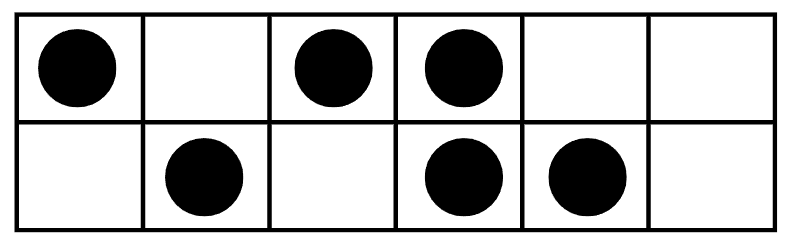
\includegraphics[width=300px]{tilings.png}
    \caption{Ejemplo para $n = 3$. Su traducción sería $((0, 1), (1, 0), (0, 1), (1, 1), (1, 0), (0, 0))$.}
    \label{fig:tiling}
\end{figure}

Como paso transitorio (y crucial), veamos que, suponiendo la existencia de exactamente $0 \leq r \leq n$ pares $(0, 0)$, entonces el resto del reparto cumple\footnote{Dicho sea de paso, y aunque pueda resultar obvio bajo la mirada de cualquier pensador crítico, las mentes menos beneficiadas por el azar agradecerán saber que en cada fila hay $n$ casillas ocupadas y otras $n$ libres.}: $r$ pares $(1, 1)$, $n - r$ pares $(0, 1)$ y $n - r$ pares $(1, 0)$.
Al haber $r$ pares $(0, 0)$, en la fila superior (o la inferior, el argumento es simétrico) quedan precisamente $n - r$ celdas libres que deben situarse ``sobre'' una ocupada de la fila baja, pues de no ser así crecería el número de pares $(0, 0)$. Esto prueba el cardinal de pares $(0, 1)$.

El proceso deductivo del párrafo anterior nos deja $r$ celdas ocupadas aún por ``emparejar'', cada una de las cuales, luego de razonar brevemente, deben ir situadas bajo otra celda ocupada, lo cual zanja también los $(1, 1)$. Y, por último, sin tener más remedio, los $n - r$ pares restantes se ven obligados a ser $(1, 0)$.

Para concluir, tras probar este \textit{lema transitorio}, vuestro sistema nervioso central no se pondrá conflictivo para aceptar la biyección entre \eqref{eq:eq001} y \eqref{eq:eq002}. Pues nada, una nueva aventura en la que resultamos invictos llega a su fin. \hfill{\textsc{T.h.e.E.n.d.}}

\end{document}
